
\documentclass[9pt]{beamer}
%\makeatletter
%\def\beamer@calltheme#1#2#3{%
%	\def\beamer@themelist{#2}
%	\@for\beamer@themename:=\beamer@themelist\do
%	{\usepackage[{#1}]{\beamer@themelocation/#3\beamer@themename}}}
%
%\def\usefolder#1{
%	\def\beamer@themelocation{#1}
%}
%\def\beamer@themelocation{}

%\usefolder{../config}

\usetheme[
block=fill,
titleformat=regular,
progressbar=frametitle
]{metropolis}
%\metroset[everytitleformat=regular] % regular, lowercase, uppercase ]
%\metroset[inner/block=fill]

%\setbeameroption{show notes} 
\usepackage{booktabs}
\usepackage[scale=2]{ccicons}

\usepackage{pgfplots}
\usepgfplotslibrary{dateplot}


%\ Hrvatski znakovi
\usepackage[utf8]{inputenc}
\usepackage[T1]{fontenc}
\usepackage[croatian]{babel}
\usepackage{todonotes}
\usepackage{amsmath}
\usepackage{amsfonts}
\selectlanguage{croatian} % american ngerman
\usepackage{todonotes}

% Koristenje Latin modern fonta
% Bez toga na nekim racunalima baca
% err: Font <taj i taj> at <mala velicina, npr4.0pt> not loadable: Metric (TFM) file not found. \end{frame}
\usepackage{lmodern}


\definecolor{RoyalBlue}{cmyk}{1, 0.50, 0, 0}
%\usepackage{natbib}
%\usepackage{bibentry}
\usepackage{scrextend}
\usepackage{hyperref}
%\usepackage[pdfa=true]{hyperref}
\hypersetup{%
    %draft, % = no hyperlinking at all (useful in b/w printouts)
    %colorlinks=true, 
    linktocpage=true, pdfstartpage=3, pdfstartview=FitV,%
    % uncomment the following line if you want to have black links (e.g., for printing)
    %colorlinks=false, linktocpage=false, pdfborder={0 0 0}, pdfstartpage=3, pdfstartview=FitV,% 
    breaklinks=true, pdfpagemode=UseNone, pageanchor=true, pdfpagemode=UseOutlines,%
    plainpages=false, bookmarksnumbered, bookmarksopen=true, bookmarksopenlevel=1,%
    hypertexnames=true, pdfhighlight=/O,%nesting=true,%frenchlinks,%
    %urlcolor=webbrown, linkcolor=RoyalBlue, citecolor=webgreen, %pagecolor=RoyalBlue,%
    %urlcolor=Blue, linkcolor=Blue, citecolor=Red, %pagecolor=Black,%
    %pdftitle={\myTitle},%
    %pdfauthor={\textcopyright\ \myName, \myUni, \myFaculty},%
    pdfsubject={},%
    pdfkeywords={},%
    pdfcreator={pdfLaTeX},%
    pdfproducer={LaTeX with hyperref and classicthesis}, %
    unicode = true 
} 

%\usepackage[pdftex]{graphicx}
% declare the path(s) where your graphic files are
\graphicspath{{./}{./figures/}}


\newcommand{\executeiffilenewer}[3]{%
	\ifnum\pdfstrcmp{\pdffilemoddate{#1}}%
	{\pdffilemoddate{#2}}>0%
	{\immediate\write18{#3}}\fi%
}
\newcommand{\includesvg}[1]{%
	\executeiffilenewer{#1.svg}{#1.pdf}%
	{inkscape -z -C --file=#1.svg %
		--export-pdf=#1.pdf --export-latex}%
	\input{#1.pdf_tex}%
}


% http://tex.stackexchange.com/questions/83882/how-to-highlight-python-syntax-in-latex-listings-lstinputlistings-command

\usepackage{listings}
\usepackage{color}
\usepackage[semibold]{sourcecodepro}

% Default fixed font does not support bold face
\DeclareFixedFont{\ttb}{T1}{txtt}{bx}{n}{12} % for bold
\DeclareFixedFont{\ttm}{T1}{txtt}{m}{n}{12}  % for normal
% Custom colors
\definecolor{deepblue}{rgb}{0,0,0.5}
\definecolor{deepred}{rgb}{0.6,0,0}
\definecolor{deepgreen}{rgb}{0,0.5,0}


% Python style for highlighting
\newcommand\pythonstyle{\lstset{
		language=Python,
		basicstyle=\small\ttfamily,
		otherkeywords={self},             % Add keywords here
		keywordstyle=\small\ttfamily\color{deepblue},
		emph={MyClass,__init__},          % Custom highlighting
		emphstyle=\small\ttfamily\color{deepred},    % Custom highlighting style
		stringstyle=\color{deepgreen},
		frame=tb,                         % Any extra options here
		showstringspaces=false            % 
	}}
	
	
	% Python environment
	\lstnewenvironment{python}[1][]
	{
		\pythonstyle
		\lstset{#1}
	}
	{}
	
	% Python for external files
	\newcommand\pythonexternal[2][]{{
			\pythonstyle
			\lstinputlisting[#1]{#2}}}
	
	% Python for inline
	\newcommand\pythoninline[1]{{\pythonstyle\lstinline!#1!}}

% \includeonlyframes{current}

%\documentclass[ucs]{beamer}
%\usetheme[menuwidth={0.3\paperwidth}]{erlangen}
%\setbeamercovered{transparent=20} 

\usepackage{amsmath,amsfonts,amsthm,amssymb}
\usepackage{setspace}
\usepackage{Tabbing}
\usepackage{fancyhdr}
\usepackage{lastpage}
\usepackage{extramarks}
\usepackage{chngpage}
\usepackage{soul,color}
\usepackage{graphicx,float,wrapfig}
\usepackage{xcolor}
\usepackage[normalem]{ulem}
\usepackage{mathtools}

\definecolor{erlangenlyellow}{RGB}{123, 25, 121}
%\usepackage[utf8x]{inputenc}
%\usepackage{default}
%\usepackage[T1]{fontenc}

\usepackage{verbatim}
\usepackage{listings}


\usepackage{subcaption}
\usepackage{lmodern}

\title{Boje i sjenčanje}

% \subtitle{ Yet, it doesn't seem so clear to me anymore…?}
\subtitle {And all things lead to here; where the crimson veil descends}
\institute{Računalna grafika}


\begin{document}
\begin{frame}
 \titlepage
\end{frame}

%\begin{frame}{Sadržaj}
%  \tableofcontents
%  % You might wish to add the option [pausesections]
%\end{frame}
% \section{Uvod}
\section{Boje}
\begin{frame}{Boje}
	\begin{block}{Ukratko o bojama i ostalom}
		\begin{itemize}
			\item Boja objekta ovisi o samom objektu, svjetlosnom izvoru, bojama okoline i čovjekovom vizualnom sustavu. 	
			\item Boje se uglavnom koriste u kvalitativnom, a ne u kvantitativnom smislu
			\item Neki objekti reflektiraju svjetlo, dok ostali propuštaju svjetlo
			\begin{itemize}
				\item Površina koja reflektira samo plavu svjetlost, postaje crna ako se osvijetli crvenim svjetlom
				\item Zeleno svjetlo postaje crno ako se promatra kroz staklo koje propušta samo crveno svjetlo
			\end{itemize}
			\item Osjet boje
			\begin{itemize}
				\item Fizikalne osobine: Vidljivi dio svjetla se sastoji od elektromagnetskog spektra koje oko može detektirati (380nm - 740 nm)
				\item Psihološka interpretacija signala - svjetlo nema boju.
			\end{itemize}
		\end{itemize}
	\end{block}
\end{frame}

\begin{frame}{Akromatsko svjetlo}
	\begin{block}{Akromatsko svjetlo}
		\begin{itemize}
			\item Intenzitet svjetla(\textsl{intensity, luminance}) - psihološki osjećaj
			\item Nivoi sive boje : (0.0-1.0)
		\end{itemize}
		
		\begin{center}
			
\includegraphics[height=1cm]{slike/mach_banding.png}
		\end{center}
		\begin{itemize}
			\item Oko je osjetljivije na male promjene intenziteta nego na male promjene boje(\textsl{hue})
		\end{itemize}
		
		\begin{center}
			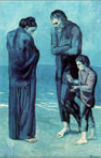
\includegraphics[height=2cm]{slike/poor_people_blue.png}\ 
			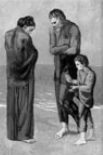
\includegraphics[height=2cm]{slike/poor_people_gray.png}
		\end{center}
	\end{block}
\end{frame}

\begin{frame}{Osnovne postavke osjeta boje}
	\begin{itemize}
		\item Svjetlina, (\textsl{brightness})
		\item Boja:
		\begin{itemize}
			\item Nijansa boje,\textsl{Hue} - položaj u spektru - kut u polarnim koordinatama
			\item Zasićenje, \textsl{Saturation} - polumjer u polarnim koordinatama
		\end{itemize}
	\end{itemize}
\end{frame}

\begin{frame}{Vidljivi spektar}
	\begin{center}
		%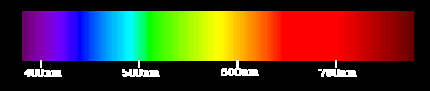
\includegraphics[height=1.5cm]{slike/02_vidljivi_spektar2.png}
		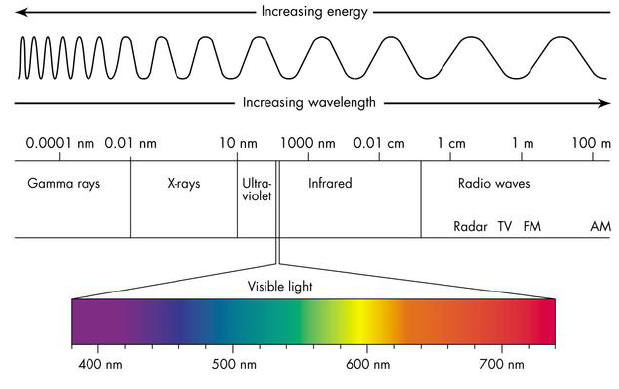
\includegraphics[height=4cm]{slike/spektar.png}
	\end{center}
	\begin{center}
		\begin{tabular}{ll}\hline
			spektralna boja & valna duljina\\\hline
			ljubičasta & 380-450\\
			plava & 450-500\\
			zelena & 500-570\\
			žuta & 570-590\\
			narančasta & 590-610\\
			crvena & 610-748 
		\end{tabular}
	\end{center}
\end{frame}

\begin{frame}{Percepcija boje}
	
	\only<1>{
		\begin{itemize}
			\item Čovjekova rožnica ima tri vrste čunjastih stanica. 
			\item Svaka vrsta reagira na različit spektar valnih duljina.
			\item Percepcija boje je u potpunosti proizvoljan proizvod živčanog sustava.
		\end{itemize}
	}
	\only<1>{
		\begin{center}
			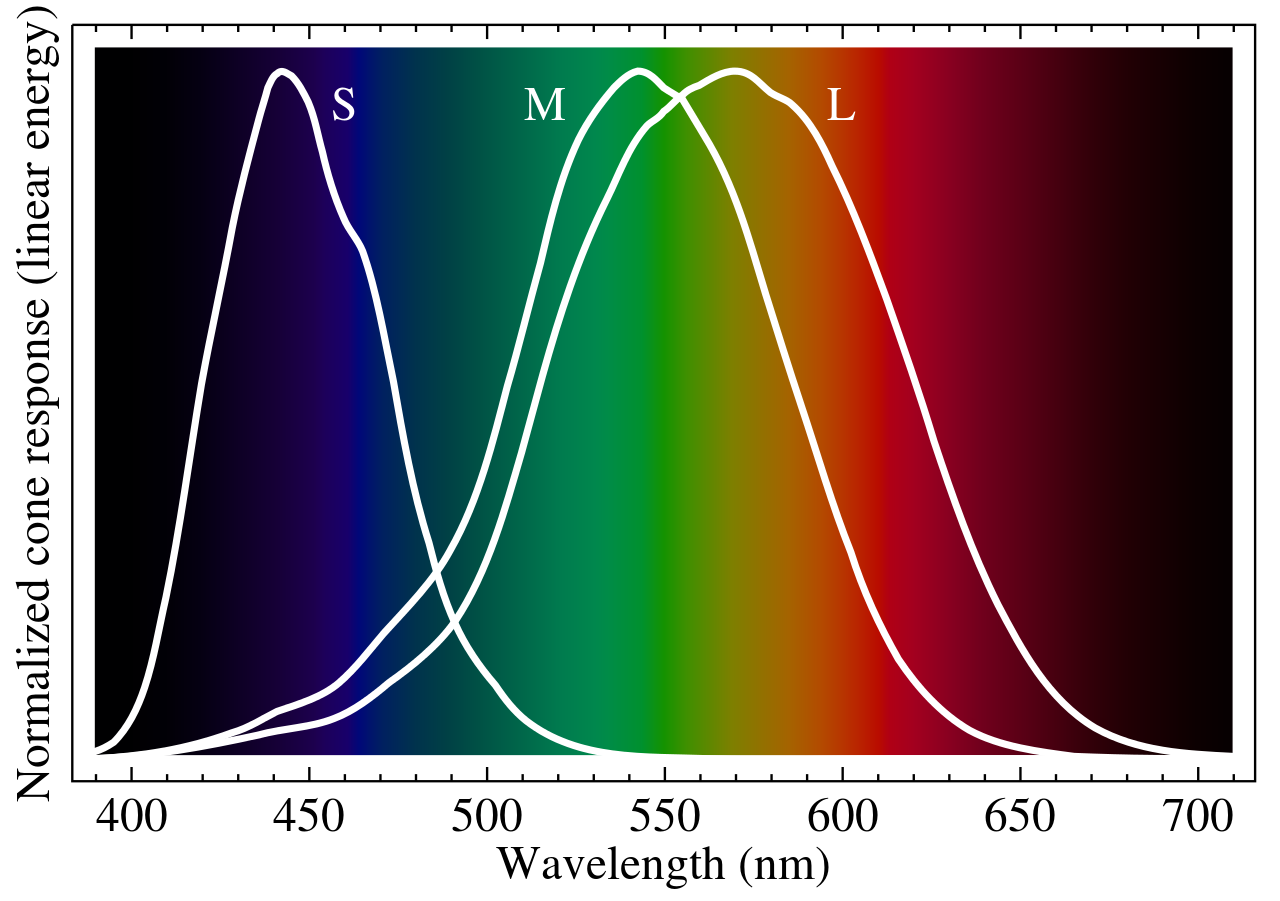
\includegraphics[width=4cm]{slike/02_cones1.png}
		\end{center}
		Crvena 500 - 700 nm, Zelena 450 - 630 nm, Plava 400 - 500 nm}
	
	\only<2>{
		\begin{center}
			Ustonožac, ili \textsl{mantis shrimp}\\
			\medskip
			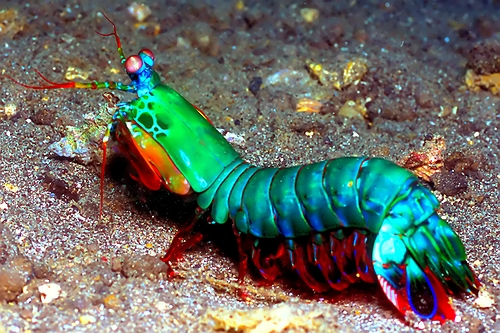
\includegraphics[width=4cm]{slike/Mantis-shrimp.jpg}
		\end{center}
	}
	\only<3>{
		\begin{center}
			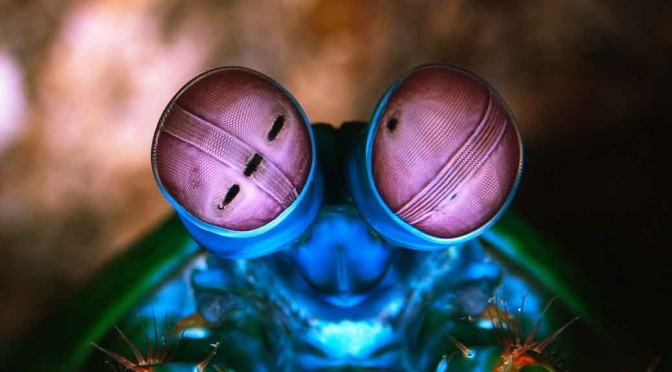
\includegraphics[width=4cm]{slike/mantis-shrimp-eyes.jpg}
		\end{center}
		\begin{itemize}
			\item dvanaest vrsta fotoreceptorskih stanica
			\item cca 300 - 700 nm
		\end{itemize}
		\begin{center}
			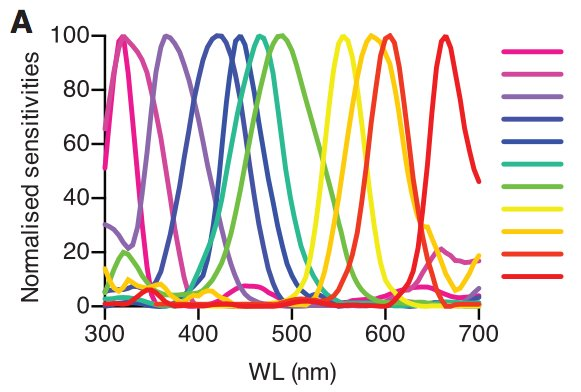
\includegraphics[width=4cm]{slike/mantis-shrimp-range.jpg}
		\end{center}
	}
\end{frame}

\begin{frame}{Percepcija boje contd.}
	\begin{itemize}
		\item Ljudi, opet
		\item Metameri su dva različita spaktra koji potiču isti odgovor
		\item Dva izvora svjetla sa različitim spektralnim distribucijama se mogu činiti kao ista boja

		\item Prisutnost tri vrste stanica: Tri parametra opisuje sve boje	
		\item Nije potrebno reproducirati cijeli spektar
	\end{itemize}

	\begin{center}
		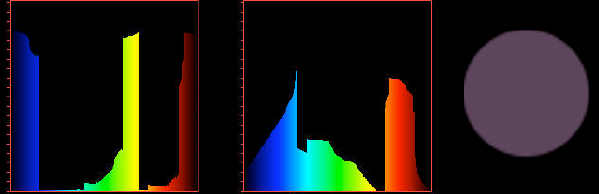
\includegraphics[height=1.5cm]{slike/02_vidljivi_spektar3.png}
	\end{center}
\begin{center}
	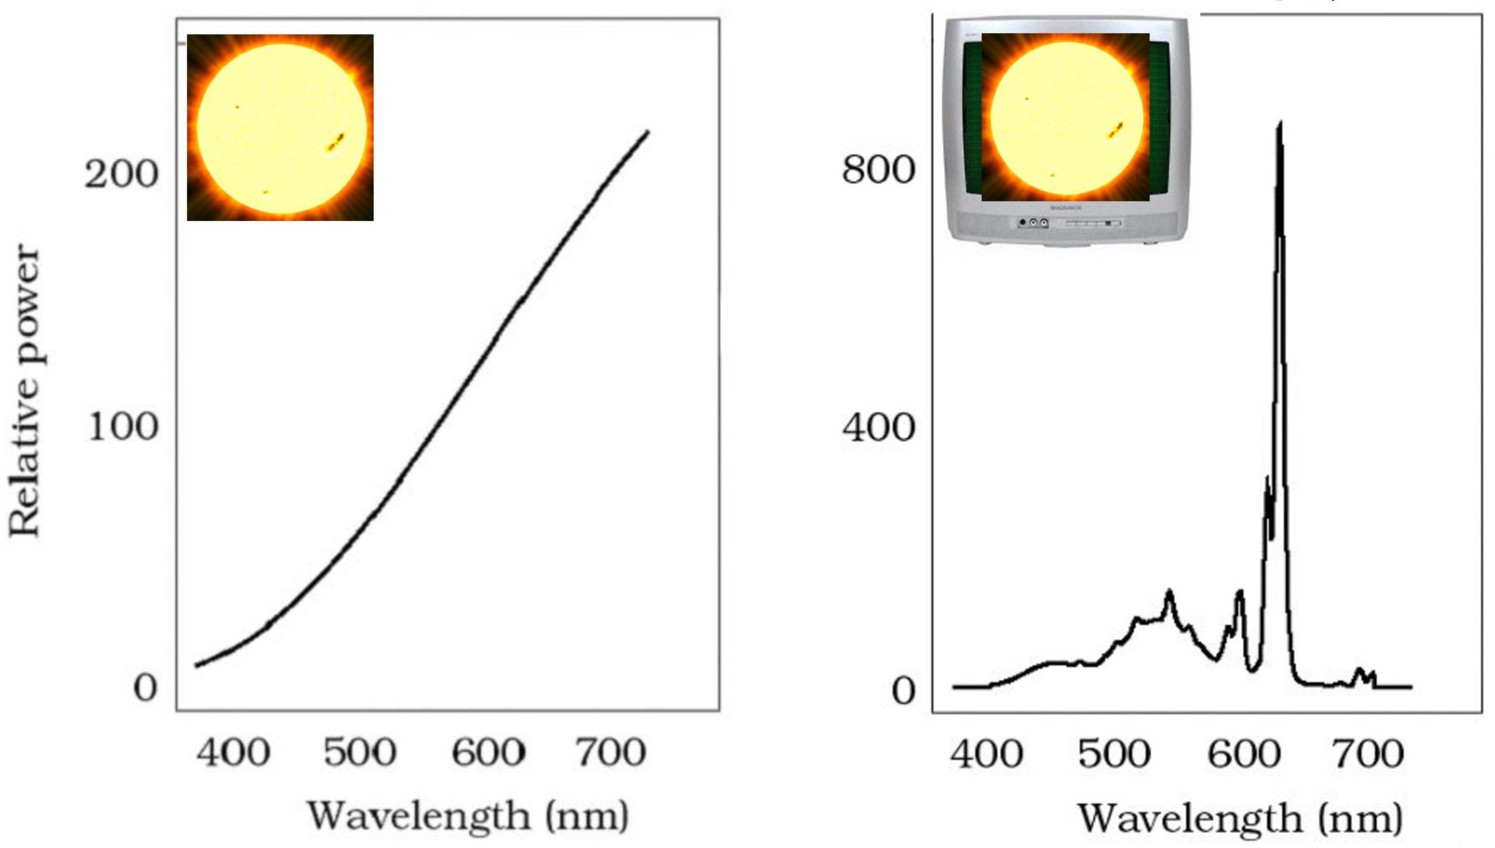
\includegraphics[height=3.5cm]{slike/color_slide_046_cropped.jpg}
\end{center}
\end{frame}

\begin{frame}{Percepcija boje contd.}
	\only<1> {
	\begin{center}
		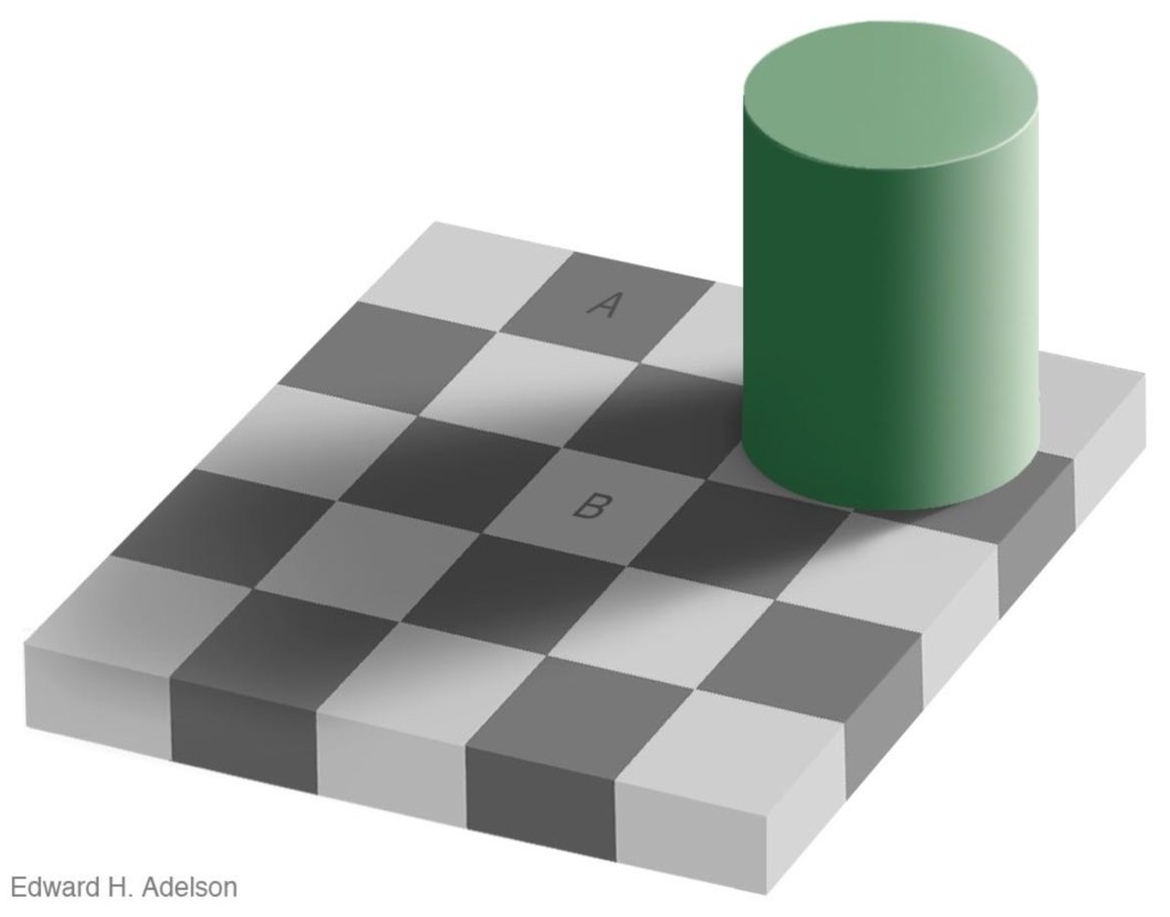
\includegraphics[height=6.5cm]{slike/color_slide_113_cropped.jpg}
	\end{center}
	}
	\only<2> {
	\begin{center}
		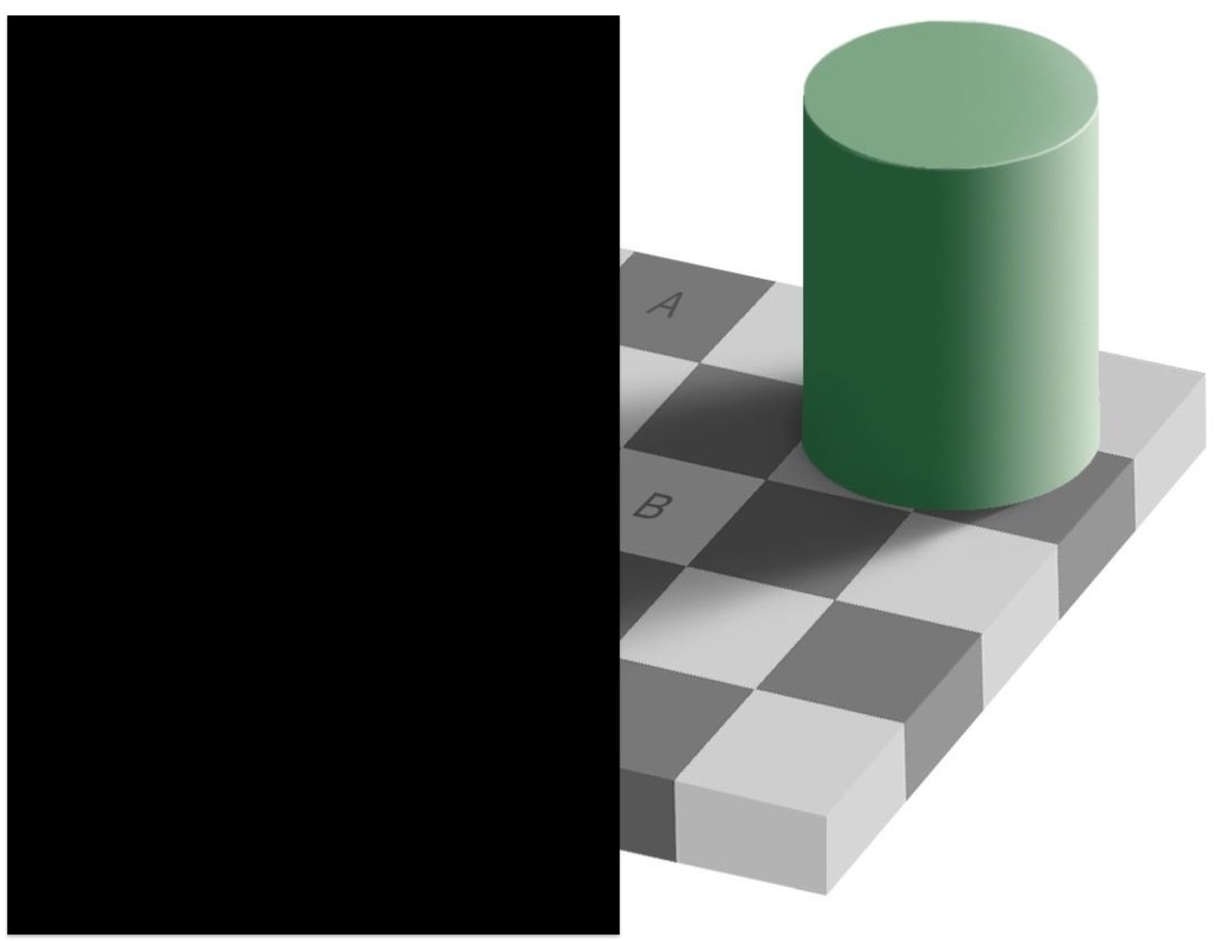
\includegraphics[height=6.5cm]{slike/color_slide_114_cropped.jpg}
	\end{center}
	}	
	\only<3> {
	\begin{center}
		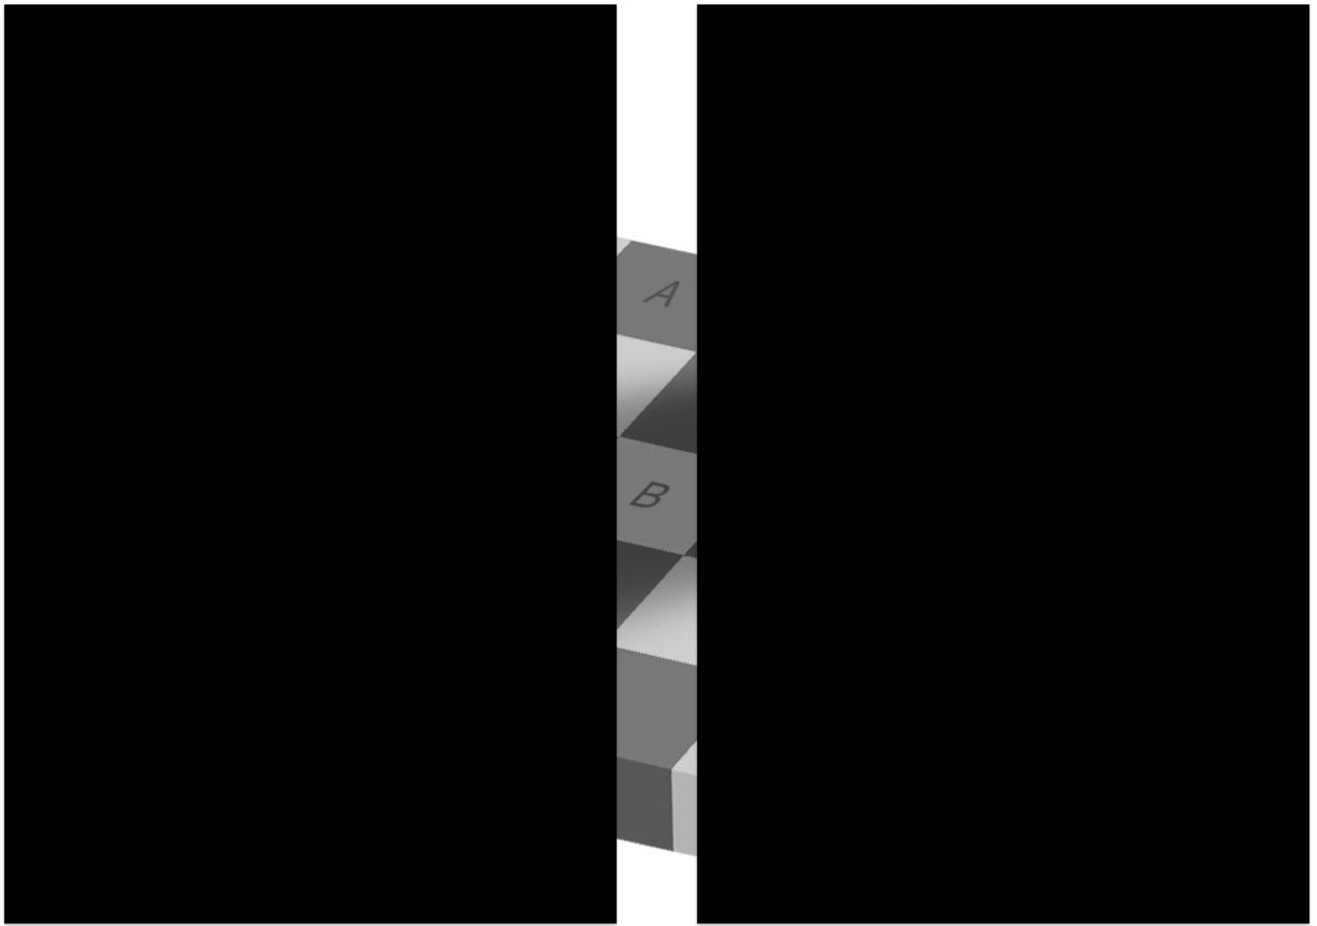
\includegraphics[height=6.5cm]{slike/color_slide_115_cropped.jpg}
	\end{center}
	}
	\only<4> {
	\begin{center}
		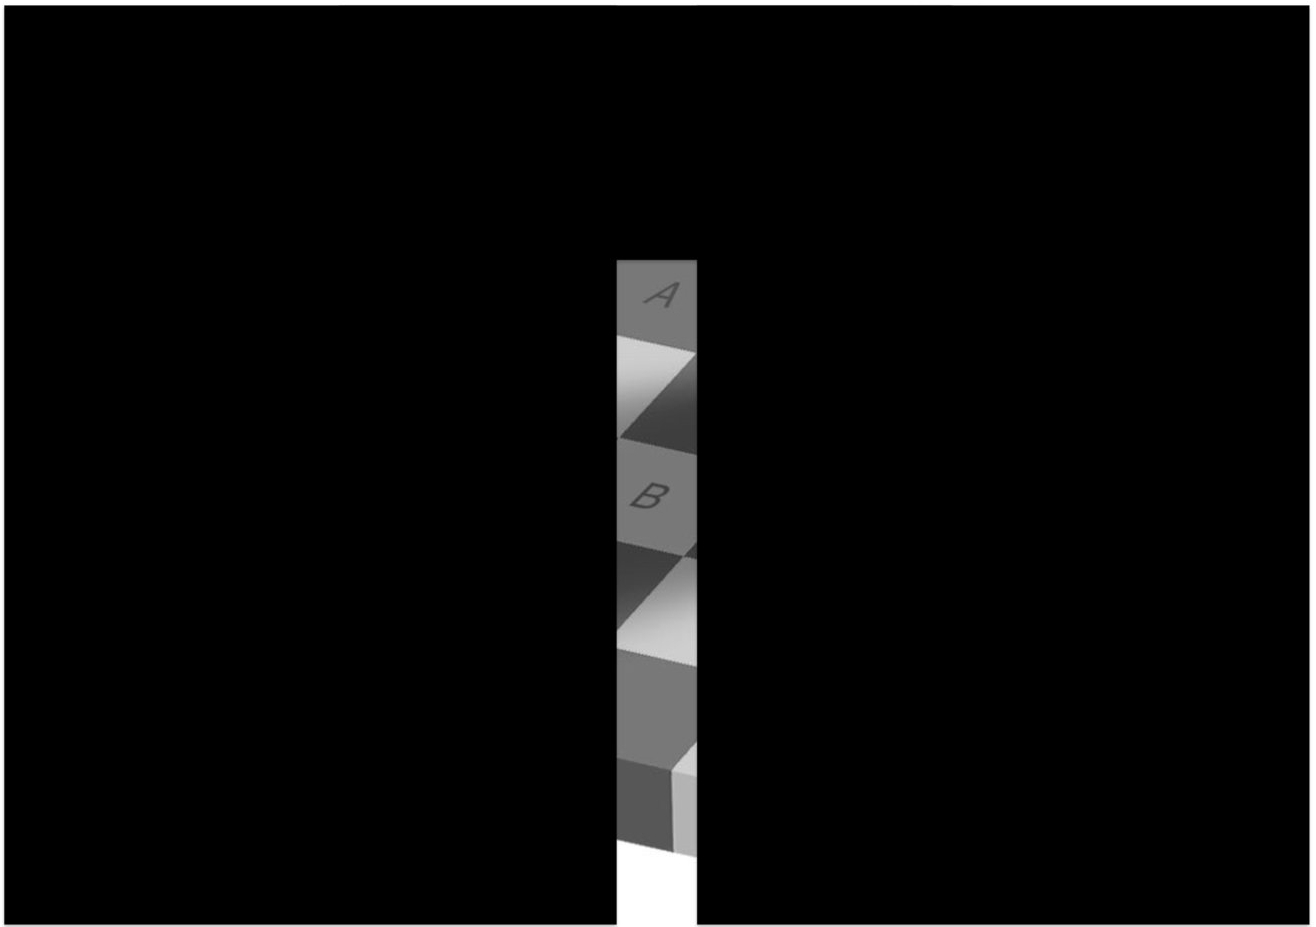
\includegraphics[height=6.5cm]{slike/color_slide_116_cropped.jpg}
	\end{center}
	}
	\only<5> {
	\begin{center}
		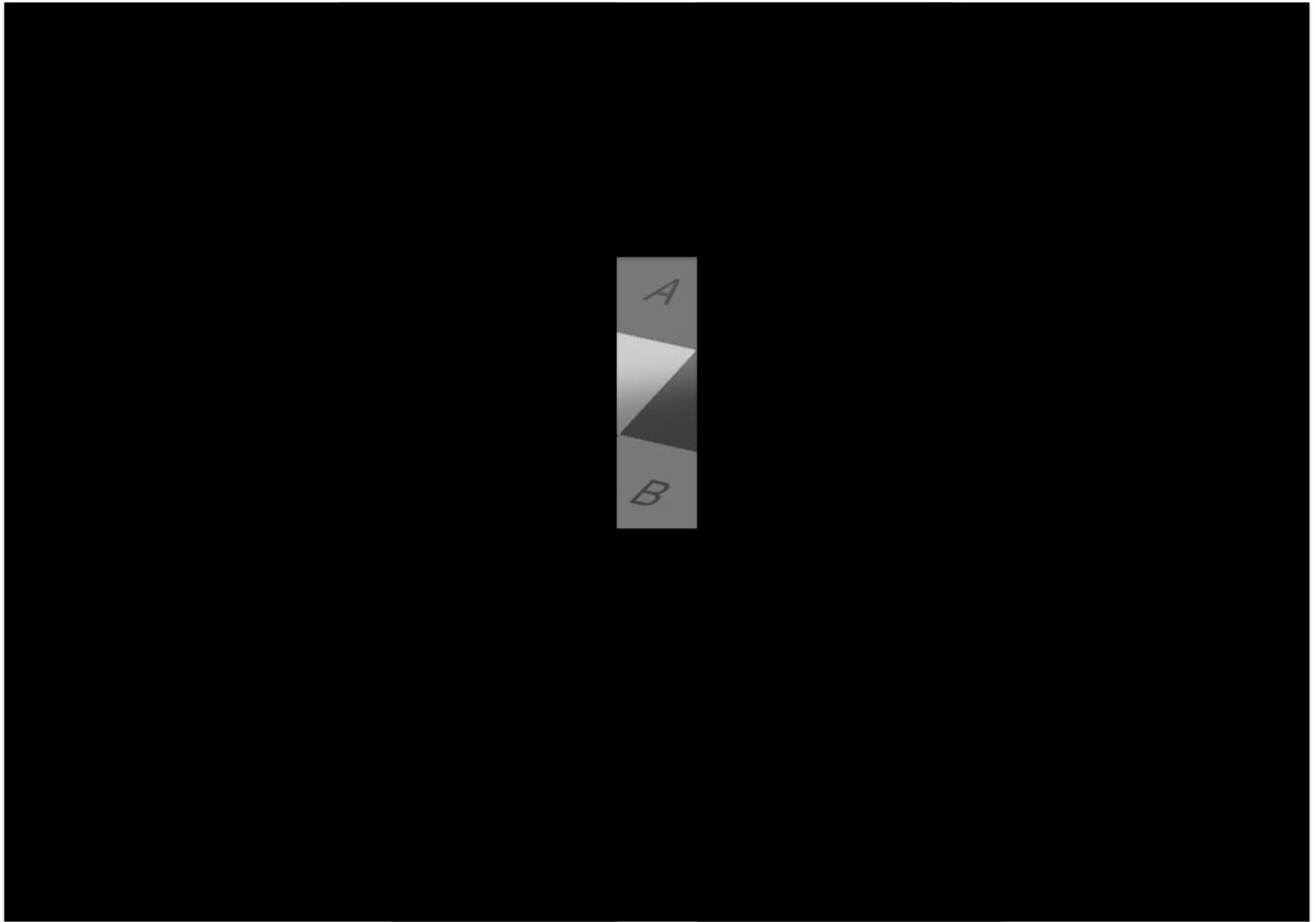
\includegraphics[height=6.5cm]{slike/color_slide_117_cropped.jpg}
	\end{center}
	}
	\only<6> {
	\begin{center}
		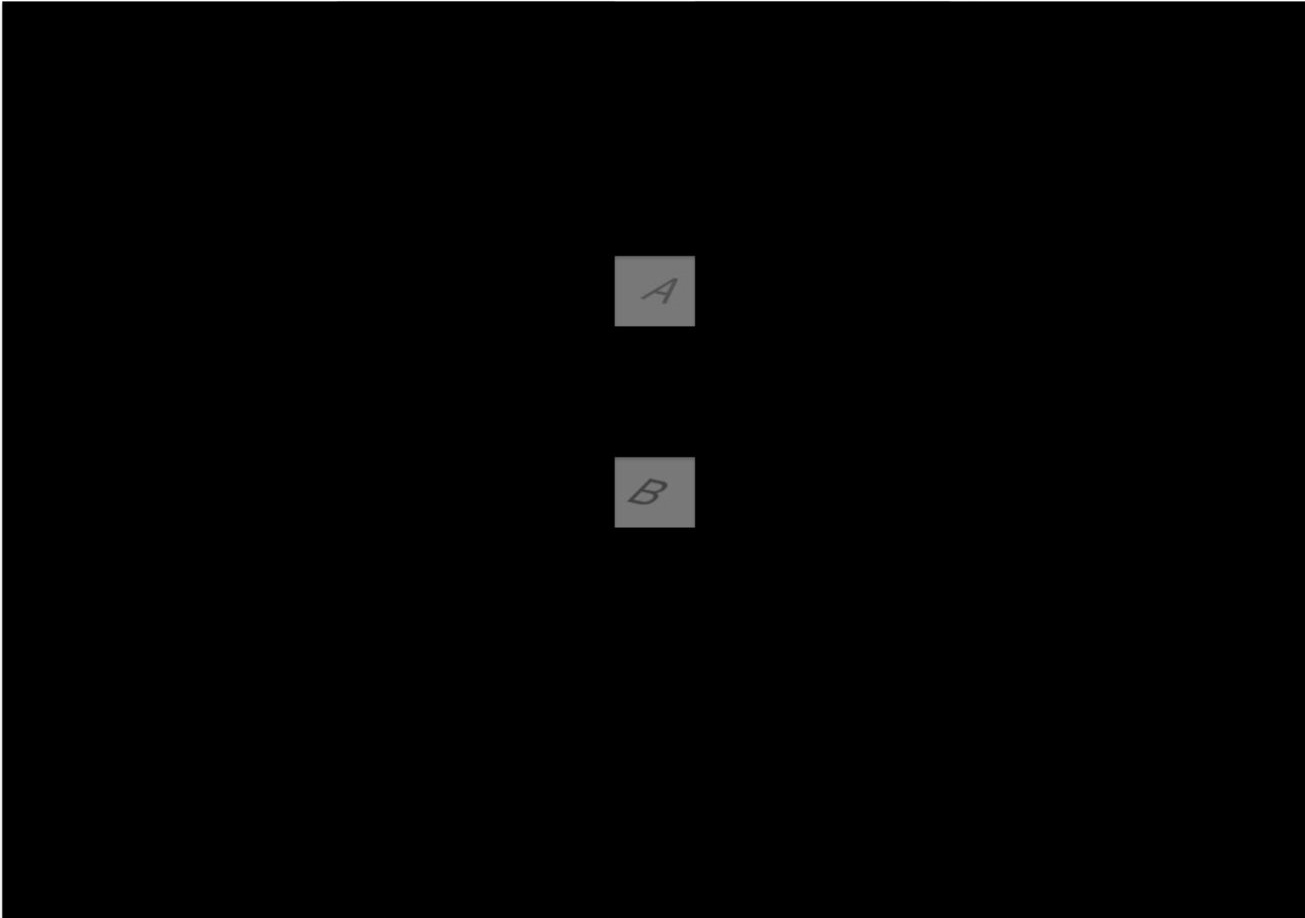
\includegraphics[height=6.5cm]{slike/color_slide_118_cropped.jpg}
	\end{center}
	}
\end{frame}	

\begin{frame}{Percepcija boje contd.}
	\only<1> {
		\begin{center}
			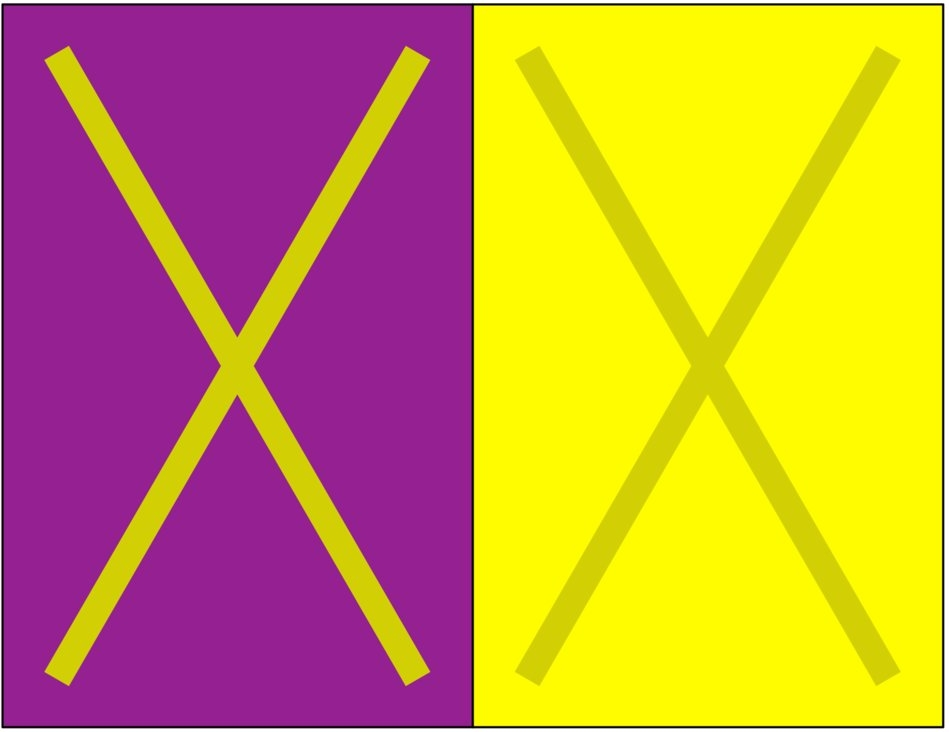
\includegraphics[height=6.5cm]{slike/color_slide_119_cropped.jpg}
		\end{center}
	}
	\only<2> {
		\begin{center}
			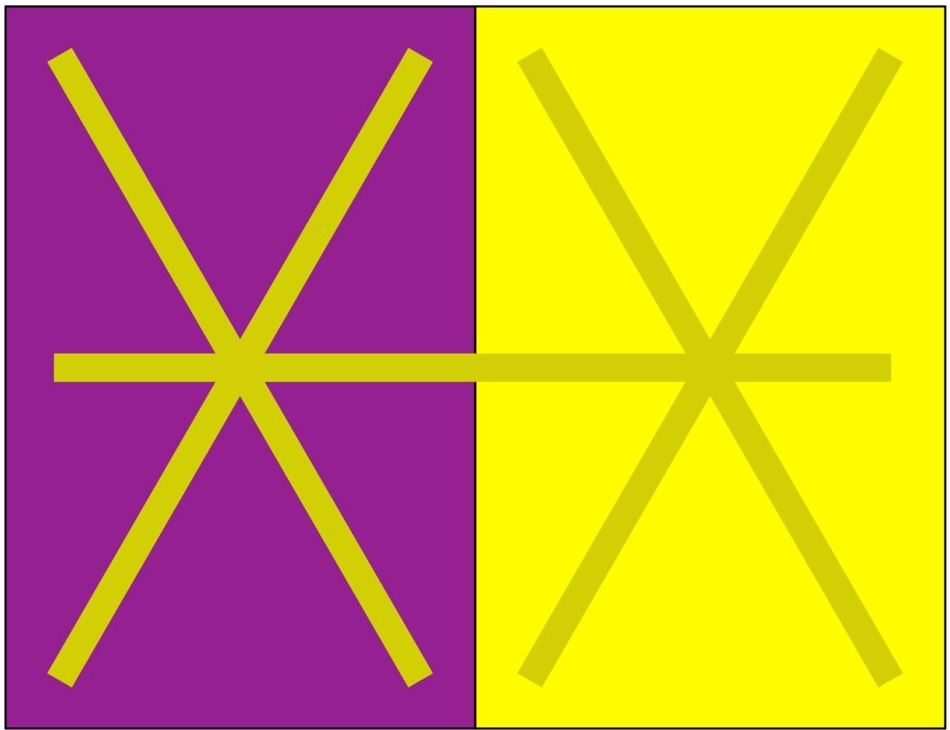
\includegraphics[height=6.5cm]{slike/color_slide_120_cropped.jpg}
		\end{center}
	}	
\end{frame}


\begin{frame}{Kako opisati sve vidljive boje}
	\begin{center}
		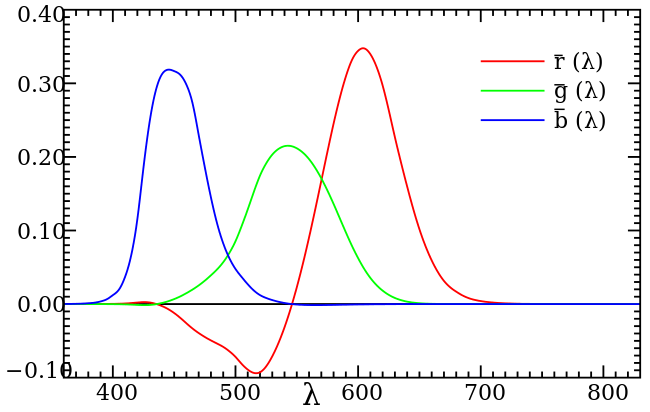
\includegraphics[height=7cm]{slike/rgb_mathcing_fun.png}
	\end{center}
\end{frame}

\begin{frame}{Kako opisati sve vidljive boje, contd.}
	\begin{itemize}
		\item Umjesto kombinacija R, G i B, uvesti X, Y i Z
		\item $X = k \int r_{\lambda} d \lambda$, itd.
		\item Uvesti  relaciju $X + Y + Z = 1$
	\end{itemize}
	\begin{center}
		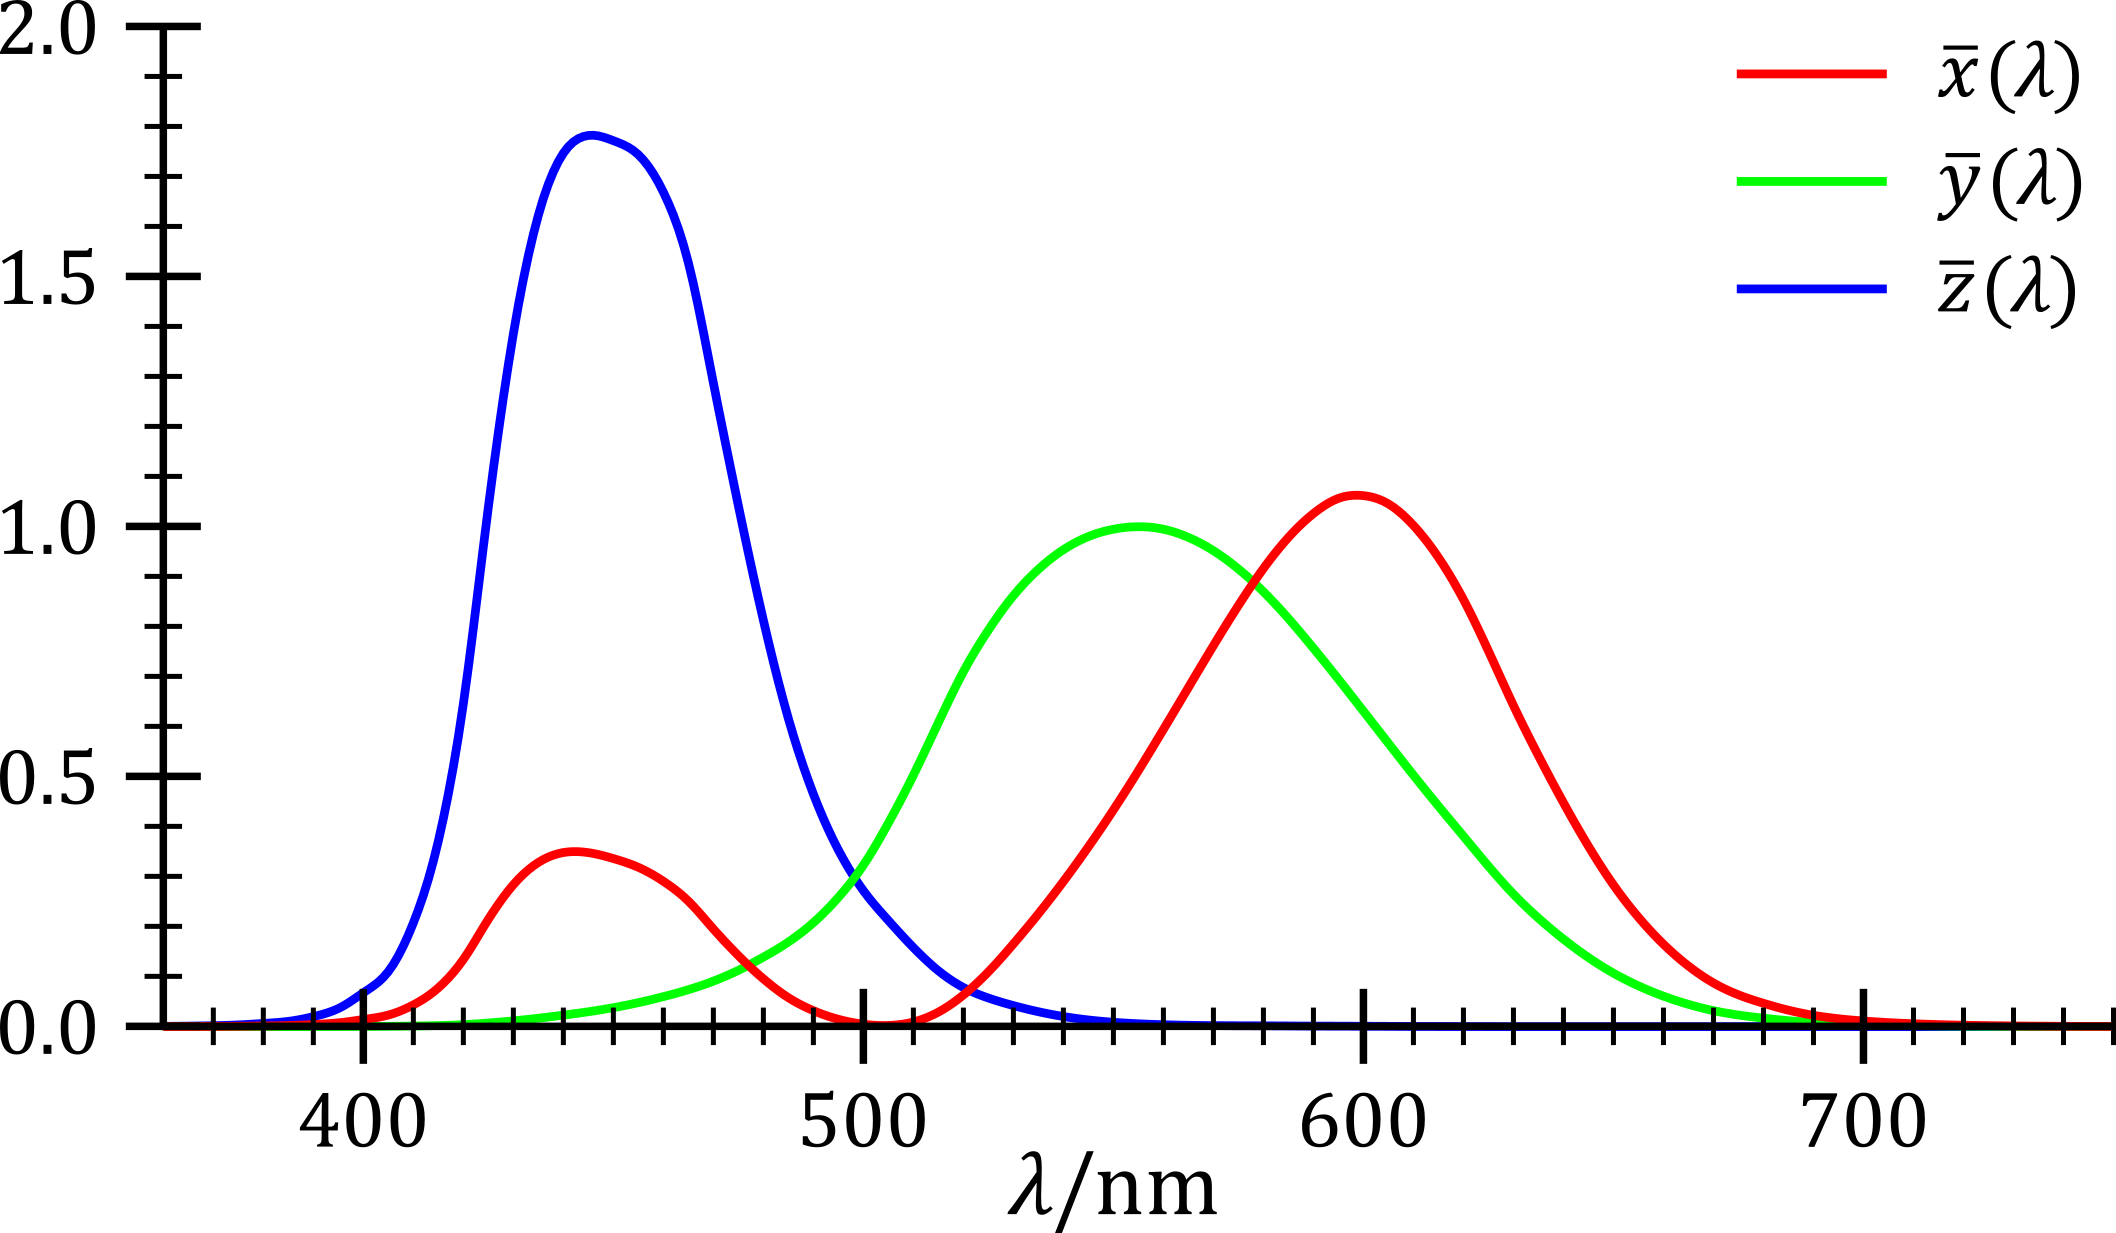
\includegraphics[height=4cm]{slike/CIE_1931_XYZ_Color_Matching_Functions.png}
	\end{center}
	\begin{align*}
	x = \frac{X}{X+Y+Z} \\
	y = \frac{Y}{X+Y+Z} \\
	z = 1-x-y
	\end{align*}
\end{frame}
\begin{frame}{CIE}
	\begin{center}
		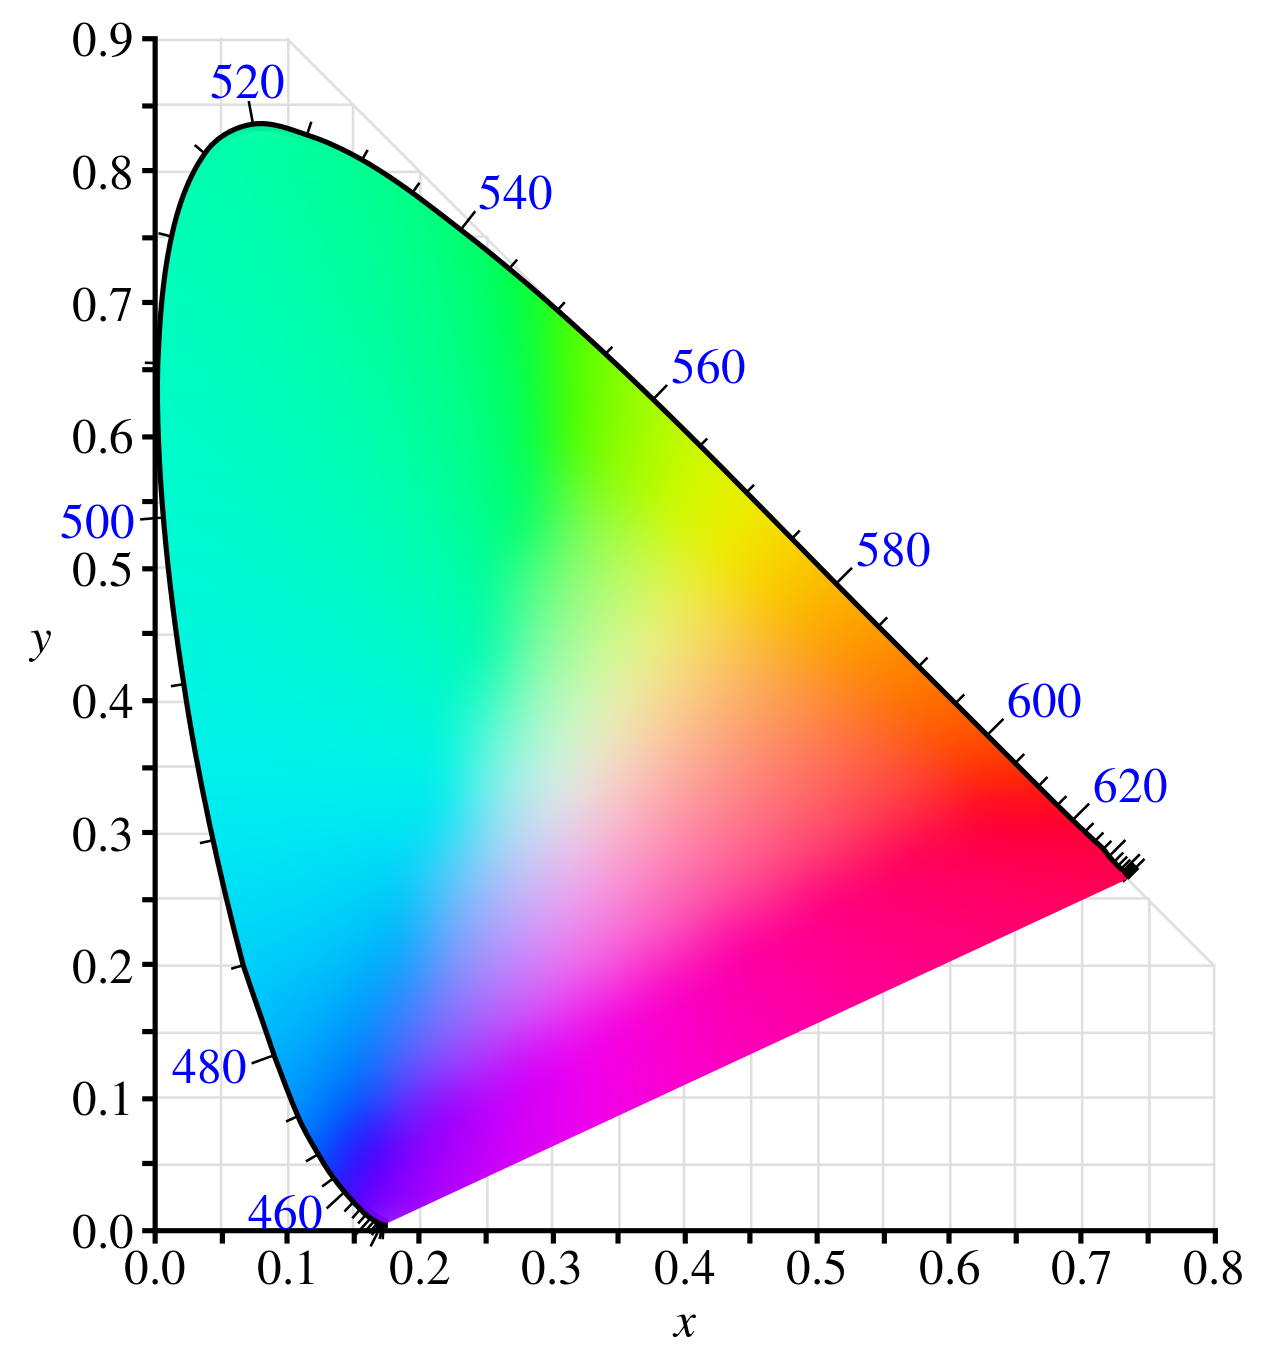
\includegraphics[height=6cm]{slike/CIE1931xy_blank.png}
	\end{center}
\end{frame}

\begin{frame}{CIE}
	\begin{center}
		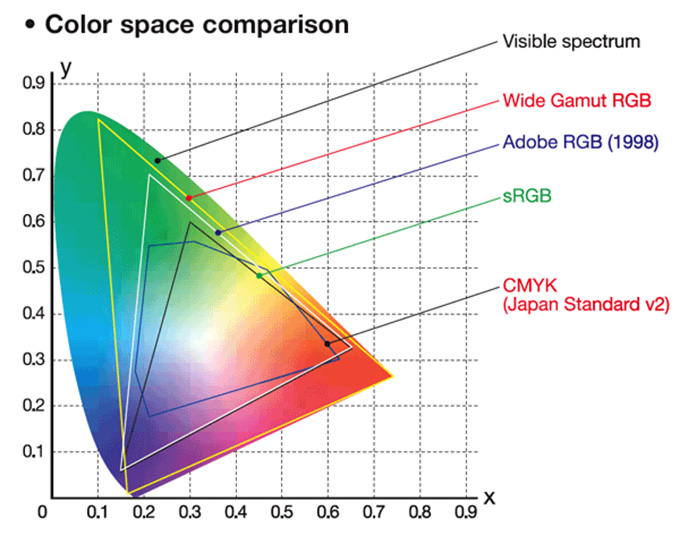
\includegraphics[height=6cm]{slike/cie_gamuts.jpg}
	\end{center}
\end{frame}

\begin{frame}{Sustavi boja}
	\begin{itemize}
		\item RGB
		\item CMYK
		\item HSV
		\item \ldots
	\end{itemize}
\end{frame}

\begin{frame}{RGB sustav}
	\begin{itemize}
		\item aditivni sustav boja
		\item smjesa tri primarne boje
		\item 256x256x256 = 16 777 216
		\item 256 razina sive boje
	\end{itemize}
	\begin{center}
		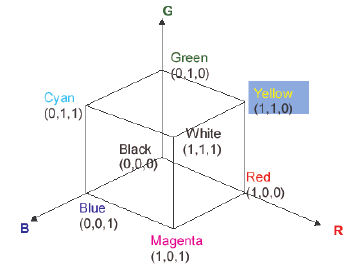
\includegraphics[height=4cm]{slike/03_rgb_01.png}
		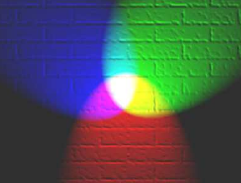
\includegraphics[height=3cm]{slike/03_rgb_02.png}
	\end{center}
\end{frame}

\begin{frame}{CMYK sustav}
	\begin{itemize}
		\item C - cyan M – magenta Y – yellow K – key
		\item subtraktivan sustav boja
		\item bijela boja je boja papira, dok je crna puna kombinacija svih tinti
		\item Boje se određuju na način da se oduzimaju od bijelog svjetla
		\item Ukoliko su filtrirane sve boje, preostaje crna
	\end{itemize}
	\begin{center}
		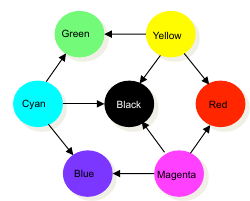
\includegraphics[height=4cm]{slike/cmyk.png}
	\end{center}
\end{frame}

\begin{frame}{HLS, HIS, HSV sustav}
	\begin{itemize}
		\item H - hue, nijansa boje, tonalnost, ime spektralne boje
		\item L - lightness, luminance svjetlina
		\item I - intensity, intenzitet
		\item S - saturation zasićenje – koliko je boju
		razrijedila bijela odnosno siva svjetlost
	\end{itemize}
	\begin{center}
		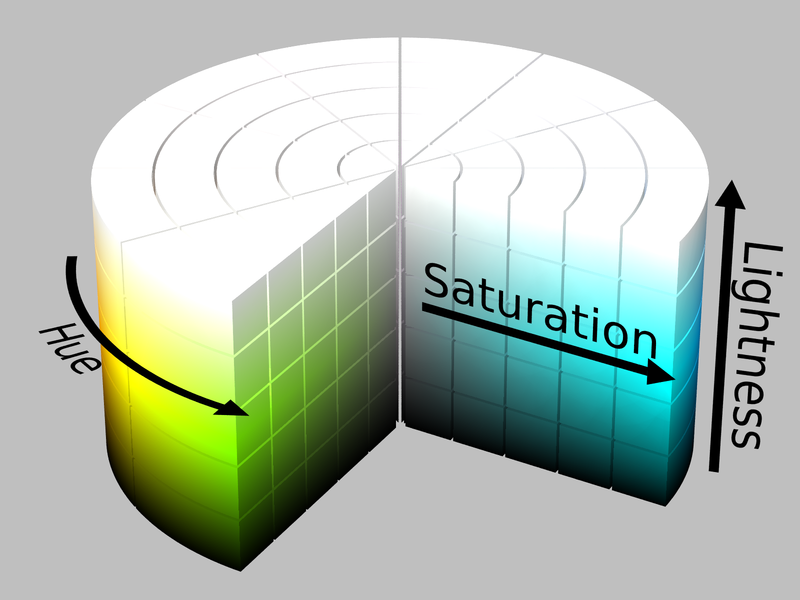
\includegraphics[height=3cm]{slike/04-hsl_color_solid_cylinder_alpha_lowgamma.png}
		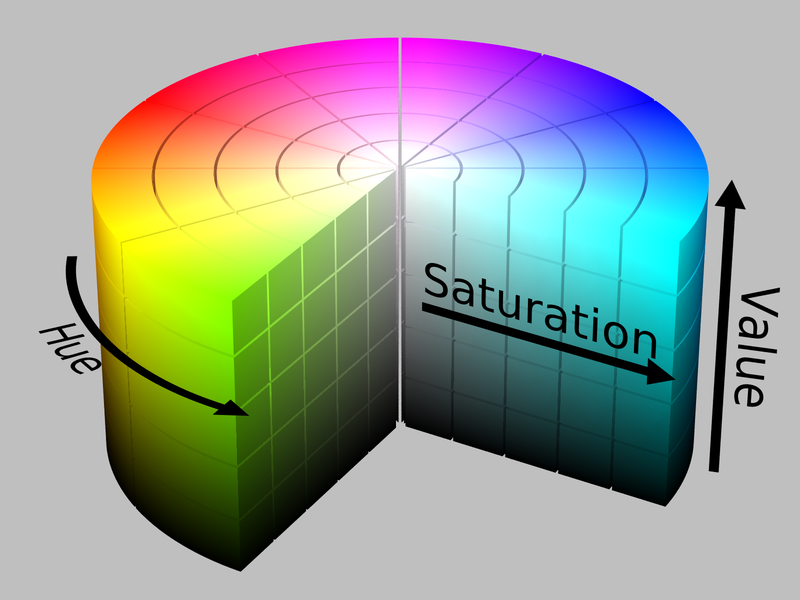
\includegraphics[height=3cm]{slike/04-hsv_color_solid_cylinder_alpha_lowgamma.png}
	\end{center}
\end{frame}

\begin{frame}{HLS, HSV sustav}
	\begin{center}
		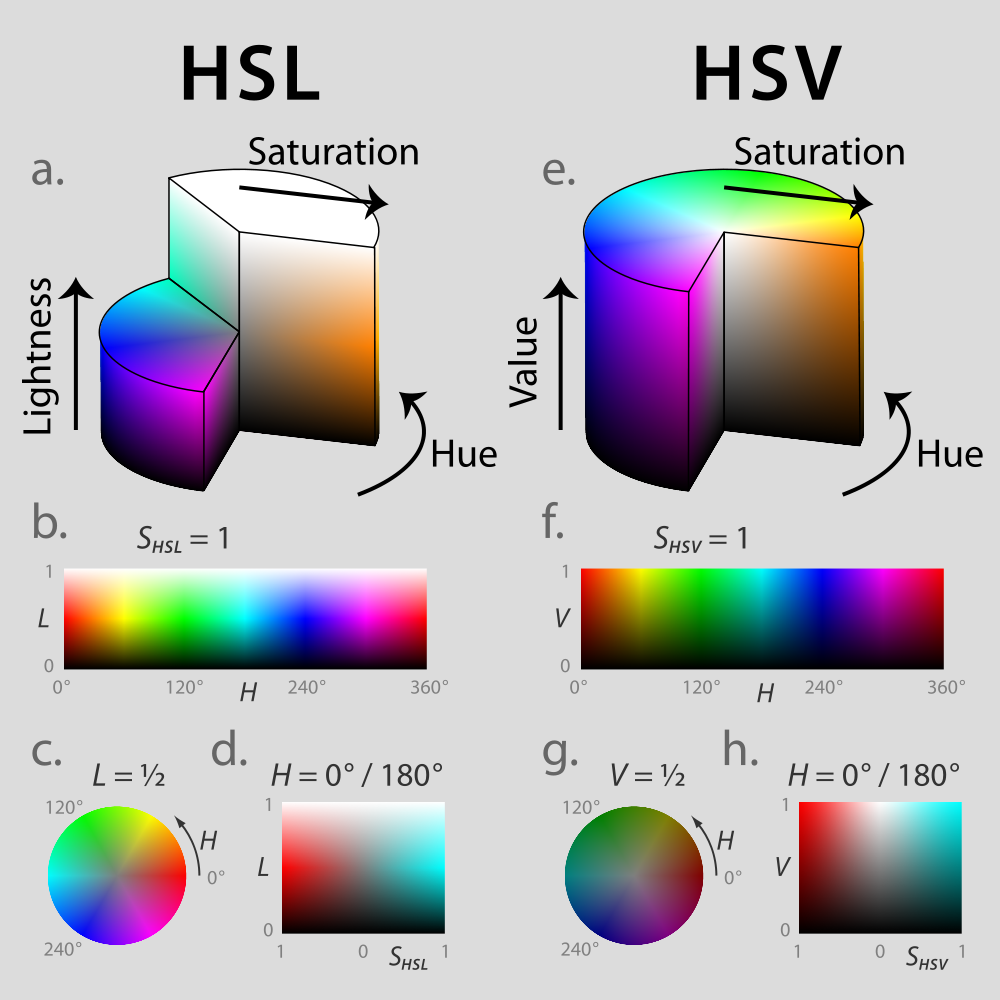
\includegraphics[height=7cm]{slike/04_hsl-hsv_models.png}
	\end{center}
\end{frame}

\begin{frame}{Sivi tonovi}
	Fotografija: svaki piksel sadrži samo intenzitet. Često su rezultat mjerenja intenziteta svjetla  dijela elektromagnetnog spektra 
	(vidljivo svjetlo, ultracrveno, ultraljubičasto\ldots)
	\begin{block}{Konverzija u grayscale}
		Potrebno je dobiti vrijednosti R, G, B kanala u linearnom intenzitetu preko gamma konverzije. Tada se dodaje 30\% na crveno, 
		59\% na zeleno i 11\% na plavo, odnosno \[Y = 0.3R + 0.59G + 0.11B\]
	\end{block}
\end{frame}

\begin{frame}{Sivi tonovi}
	\begin{center}
		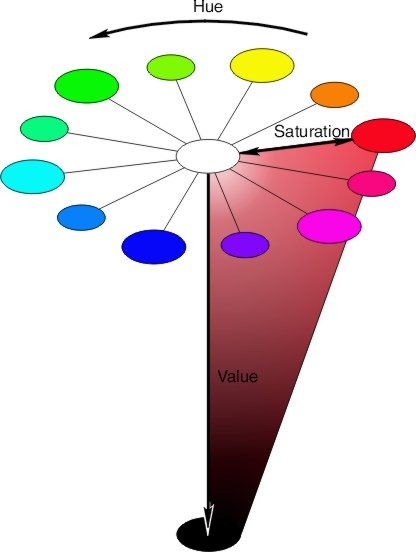
\includegraphics[height=7cm]{slike/07_hexacone-5.png}
	\end{center}
\end{frame}


\begin{frame}{Intenzitet}
	
	
	\begin{block}{Veza oka (opazive svjetline)  $S$ s mjerljivim intenzitetom $I$}
		\begin{itemize}
			\item Linearna veza podrazumijeva jednake korake u $I$ kao i u $S$
			\item Ljudski sustav se zasniva na omjerima: $I=0.1$ i $0.11$ su isti kao i $0.5$ i $0.55$
		\end{itemize}
	\end{block}
\end{frame}
\begin{frame}{Intenzitet contd.}
	
	\[S = const. \log{I}\]
	
	
	Ako želimo postići jednake korake u opazivoj svjetlini, za 255 vrijednosti I:
	\[\frac{I_{j}+1}{I_{j}}=\frac{I_{j}}{I_{j}-1}=r\]
	\[I_{0}=I_{0},\ I_{1}=rI_{0}, \ I_{2}=rI_{1}=I_{2}=r^{2}I_{0}\ldots I_{255}=r^{255}I_{0}\]
	\[r=\left (\frac{1}{I_{0}}\right )^{\frac{1}{255}}\ \textrm{za } 0\leq j \leq 255\]
	
	Za n+1 intenziteta:
	\[r=\left (\frac{1}{I_{0}}\right )^{\frac{1}{n}}\ I_{j}=I_{0}^{n-\frac{j}{n}}\]
\end{frame}

\begin{frame}{Intenzitet contd.}
	Umjesto kodiranja uniformnih koraka svjetline u slici, bolje kodirati korake percepcije - analogni TV signal i JPEG.
	\begin{itemize}
		\item Intenzitet CRT monitora je proporcionalan s naponom $V^{5/2}$ 
		\item Ekponent se još naziva $\gamma$ eksponent
		\item PC monitori imaju $\gamma = 2.5$, dok Mac ima $\gamma = 2.2$ - Mac slike su tamnije
	\end{itemize}
	
\end{frame}

\begin{frame}{Gamma korekcija}
	\begin{itemize}
		\item Definira vezu između vrijednosti piksela i intenziteta osvijetljenja.
		\item Digitalna kamera linearno skalira razinu osvjetljenja
		\begin{itemize}
			\item Alocira se previše bitova na osvjetljenje kojie ljudsko oko ne može percipirati
			\item Alocira se premalo bitova na tamnije tonove na koje je ljudsko oko najosjetljivije
		\end{itemize}
	\end{itemize}
	
	\begin{tabular}{ll}
		Original &
\includegraphics[height=0.5cm]{slike/05_gamma_gradient3b.png}\\
		Linear&  
\includegraphics[height=0.5cm]{slike/05_gamma_gradient2b.png}\\
		Gamma&  
\includegraphics[height=0.5cm]{slike/05_gamma_gradient1b.png}
	\end{tabular}
	Zaključno (opet): Oko je osjetljivije na promjene tamnih tonova nego na slične promjene svijetlih tonova.
	
\end{frame}
\begin{frame}{Gamma korekcija contd. }
	\begin{itemize}
		\item Ako se prikazuje boja dva puta tamnija od bijele (RGB $(0.5, 0.5, 0.5)$)
		\item Takva boja će biti cca četiri puta tamnija (od bijele), jer je $0.5^{2.2} \approx 0.22$
		\item Kanali se obrađuju zasebno,  
		\item RGB $(1, 0.5, 0.5)$ postaje RGB $(1, 0.22, 0.22)$
	\end{itemize}
\end{frame}

\begin{frame}{Gamma korekcije contd.}
	Gamma korekcija - korekcija prikaza monitora.
	\[ V_{out} = V_{in}^{\gamma}\]
	\begin{center}
		\begin{tabular}{ll}
			Original &
\includegraphics[height=0.5cm]{slike/05_gamma_gradient3b.png}\\
			Linear&  
\includegraphics[height=0.5cm]{slike/05_gamma_gradient2b.png}\\
			Gamma&  
\includegraphics[height=0.5cm]{slike/05_gamma_gradient1b.png}
		\end{tabular}
	\end{center}
	\begin{itemize}
		\item Linearno kodiranje koristi nedovoljno razina za opis tamnih tonova, iako ima puno više svijetlih tonova.
		\item Gamma gradijenti ditribuiraju tonove jednako po cijelom spektru (percepcijski uniformno)
		\item Image editing, boje i histogrami su zasnovani na takvim tonovima
	\end{itemize}
	
\end{frame}

\begin{frame}{Gamma korekcije contd.}
	Na Gamma kodiranu sliku je potrebno primijeniti gamma korekciju, čime se efektivno poništava na originalnu sliku.
	\begin{center}
		\begin{tabular}{ccc}
			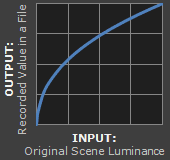
\includegraphics[height=2cm]{slike/05_gamma_chart3c.png} & 
			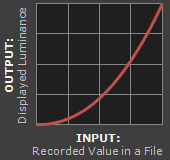
\includegraphics[height=2cm]{slike/05_gamma_chart4d.png}&
			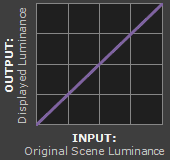
\includegraphics[height=2cm]{slike/05_gamma_chart5c.png} \\
			Image file gamma & Display gamma & System Gamma
		\end{tabular}
	\end{center}
	\begin{itemize}
		\item Image $\gamma$: Uređaj(kamera) ili RAW softver kad god se slika snima u TIFF, JPEG i sl.
		\item Display $\gamma$: Utjecaj grafičke kartice i/ili monitora - kompenzacija \textit{Image gamma}
		\item System $\gamma$: \textit{Viewing} $\gamma$, Ukupni efekt prethodnih $\gamma$ vrijednosti koje su primijenjene na sliku.
	\end{itemize}
\end{frame}

%\begin{frame}{Image Gamma}
%Obično se primjenjuje u fotoaparatu ili RAW software-u prilikom prebacivanja u jpeg ili tiff. Redistribuiraju se tonalne razine
%kamere u razine koje su percepcijski uniformne. Precizno se faktor određuje profilom boja koje se nalaze u datoteci. 
%Većina upotrebljava 1/2.2 (Adobe RGB 1998), osim RAW datoteka, koje upotrebljavaju linear gamma. RAW preglednici slika koriste 1/2.2
%\begin{center}
%\begin{tabular}{cc}
%\includegraphics[height=2cm]{slike/05_gamma_example-g10b.png} & 
%\includegraphics[height=2cm]{slike/05_gamma_example-g22b.png}\\
%Linear gamma & gamma 1/2.2
%\end{tabular}
%\end{center}
%\end{frame}

\begin{frame}{Kakva korist od korekcije}
	\begin{itemize}
		\item Dokle god slike ne napuštaju monitor, problem ne postoji 
		\item Ako slike treba tiskati, skalirati, koristiti kao teksture,
		\begin{itemize}
			\item Program treba znati da vrijednosti \textsl{nisu prave} i da su korigirane da bi 
			izgledale \textsl{for real} na monitoru
			\item Renderer koristi teksturu  i pretpostavlja da su intenziteti linearni
			\item pojednostavljeno: $A^{1/\gamma} + B^{1/\gamma} \neq (A+B)^{1/\gamma}$
			\item sumira se doprinos dvaju svjetala koji produciraju krive vrijednosti
		\end{itemize}
	\end{itemize}
	
\end{frame}

\begin{frame}{Kakva korist od korekcije}
	\begin{center}
		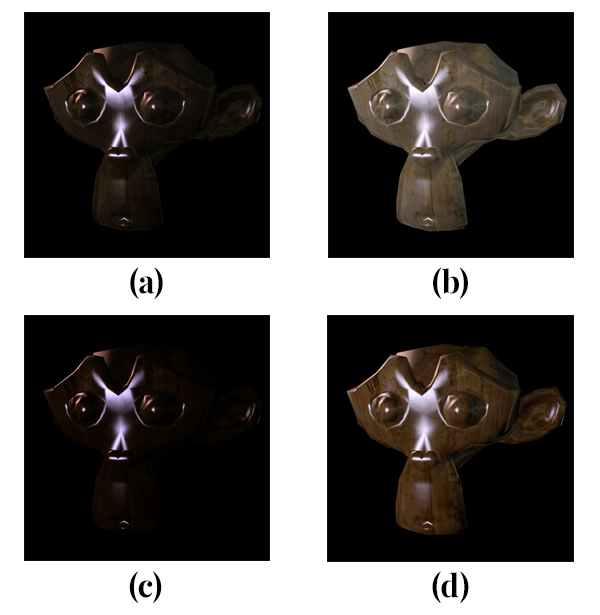
\includegraphics[height=6cm]{slike/monkey_a.png}
	\end{center}
	a) - bez korekcije teksture i završne slike 
	b) - bez korekcije teksture i s korekcijom završne slike
	c) - korekcija teksture i bez korekcije završne slike 
	d) - korekcije teksture i završne slike 
	
\end{frame}	

\section{Svjetlo}
\begin{frame}{Osvjetljavanje i materijali}
	\begin{itemize}
		\item<+-> Input za realistični render
		\begin{itemize}
			\item Geometrija, Osvjetljenje, Materijali
		\end{itemize}
		\item<+-> Materijali
		\begin{itemize}
			\item Intenzitet i oblik odsjaja
			\item Sjaj
			\item Boja
			\item Teksture
		\end{itemize}
	\end{itemize}
	\begin{center}
		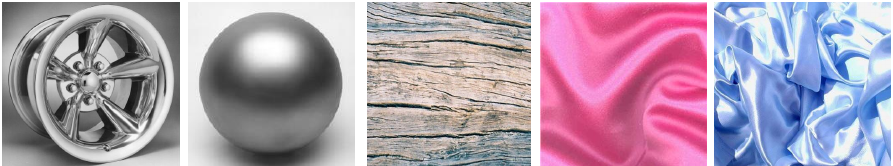
\includegraphics[height=2cm]{slike/materijali.png}
	\end{center}
\end{frame}

\begin{frame}{Točkasti izvori svjetla}
	\begin{itemize}
		\item Neočekivano, izvor svjetla je u materijalnoj točki
		\item Višestruki izvori: $I_{a+b} = I_{a} + I_{b}$
		\item Skaliranje intenzitete: $I_{sa} = sI_{a} $
	\end{itemize}
	\begin{center}
		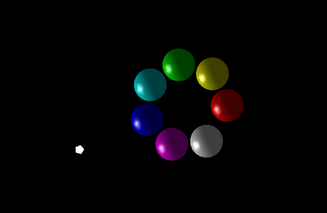
\includegraphics[height=2cm]{slike/simple_light.png}
	\end{center}
\end{frame}

\begin{frame}{Intenzitet kao funkcija udaljenosti}
	\begin{itemize}
		\item $1/r^2$ opadanje za izotropne točkaste izvore
		\item Izotropno svjetlo emitira konstantnu snagu po kutu u svim smjerovima
		\item Mora imati istu snagu u svim koncentričnim sferama
		\item Površina sfere raste s $r^2$, energija $1/r^2$
		\item $I=\infty$ za $r\rightarrow 0$
		\item Popularno: $1/(ar^2 + br +c)$
	\end{itemize}
	\begin{center}
	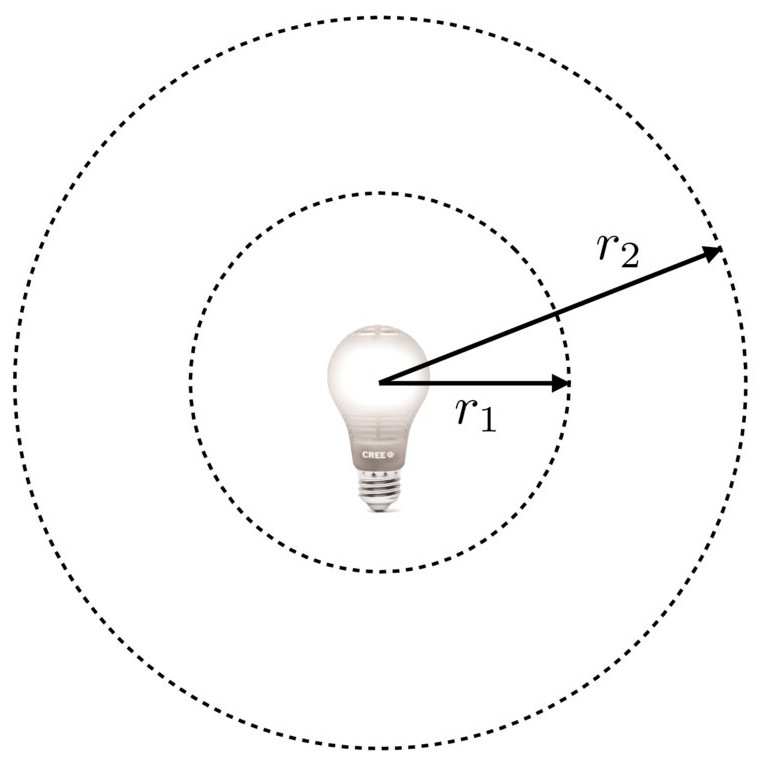
\includegraphics[height=2cm]{slike/slide_027_cropped.jpg}
\end{center}
\end{frame}

\begin{frame}{Što ako svjetlo ne pada okomito na površinu?}
	\only<1> {
		\begin{center}
			
\includegraphics[height=5cm]{slike/slide_023_cropped.jpg}
	\end{center}}
	\only<2> {
		\begin{center}
			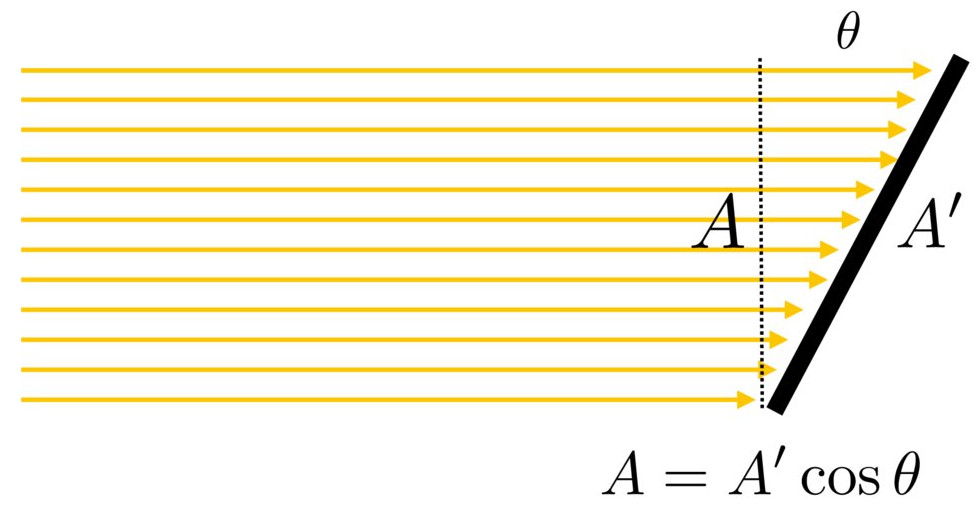
\includegraphics[height=5cm]{slike/slide_024_cropped.jpg}
	\end{center}}
	\only<3> {
		\begin{center}
			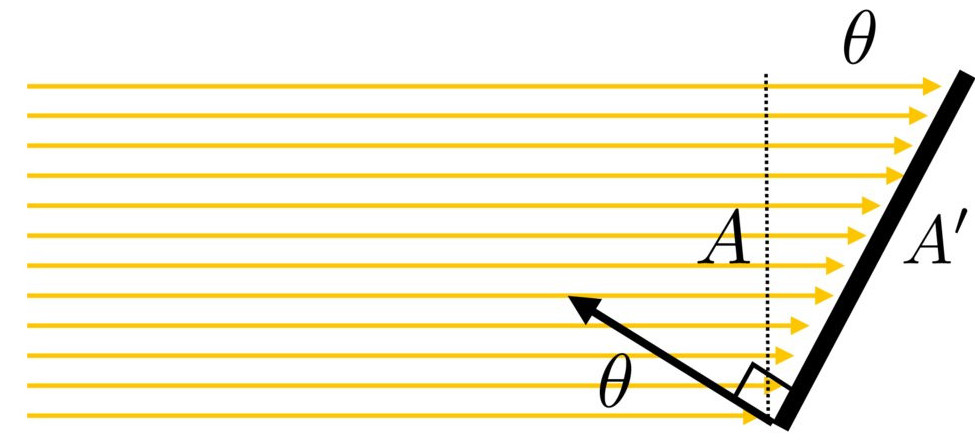
\includegraphics[height=5cm]{slike/slide_025_cropped.jpg}
	\end{center}}
\end{frame}
\begin{frame}{Zračenje\footnote[frame]{Irradiance, intenzitet}}
	\begin{itemize}
		\item Količina svjetlosne energije koja se emitira na površinu ovisi o kutu upada svjetla
		\item Veća pri normali, iako je udaljenost const.\footnote[frame]{ljeto/zima}
		\item $\cos$ zakon
		\item Skalarni produkt s normalom površine
	\end{itemize}
\end{frame}

\begin{frame}{Intenzitet}
	\begin{align*}
	I_{in} = I_{svjetlo}\frac{\cos \theta}{r^2} 
	\end{align*}
	%\begin{itemize}[<+-| alert@+>]
	\begin{itemize}
		\item $I_{in}$ Intenzitet na površini $x$
		\item $I_{svjetlo}$ Intenzitet svjetla
		\item $\theta$ Kut između zrake svjetla i $\mathbf{l}$ i normale površine $\mathbf{n}$
		\item $r$ je udaljenost od izvora svjetla do površine $x$
	\end{itemize}
\end{frame}

\begin{frame}{Intenzitet, contd.}
	\begin{itemize}
		\item Točkasti izvor svjetla koji je \alert{beskonačno} daleko
	\end{itemize}
	\begin{align*}
	I_{in} = I_{svjetlo}\cos \theta
	\end{align*}
	%\begin{itemize}[<+-| alert@+>]
	\begin{itemize}
		\item $I_{in}$ Intenzitet na površini $x$
		\item $I_{svjetlo}$ Intenzitet svjetla
		\item $\theta$ Kut između zrake svjetla $\mathbf{l}$ i normale površine $\mathbf{n}$
	\end{itemize}
\end{frame}

\begin{frame}{Spotlight}
	\begin{itemize} %[<+->]
		\item Točkasti izvor s \alert{neuniformnim} smjerom emisije svjetla
		\item Obično simetrični oko centralnog smjera $\mathbf{d}$ 
		\item Potrebno definirati i opadanje intenziteta s promjenom kuta
		\item Obično se definiraju dva kuta:
		\begin{itemize}
			\item \textsl{Hotspot} kut: Nema opadanja intenziteta svjetla unutar centralnog stošca
			\item \textsl{Falloff} kut: Intenzitet svjetla opada od punog intenziteta do nule između \textsl{Hotspot} kuta i \textsl{Falloff} kuta
		\end{itemize}
	\end{itemize}
	\begin{center}
		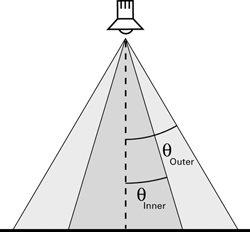
\includegraphics[height=2cm]{slike/spotlight.jpg}
	\end{center}
\end{frame}

\begin{frame}{Refleksija, BRDF}
	\begin{itemize}%[<+->]
		\item Bidirectional Reflectance Distribution Function
		\item Dvosmjerna funkcija distribucije refleksije
		\item Omjer svjetla koji dolazi iz jednog smjera koji se reflektira u drugom smjeru
		\item Čista refleksija, nema raspršivanja svjetla
		\item Usredotočenost na kut upada svjetla, a ne na varijacije površine materijala
		\item Dimenzije?
	\end{itemize}
\end{frame}

\begin{frame}{BRDF}
	\begin{itemize}
		\item 4D: dva kuta za svaki smjer
		\item $f_r(\theta_i, \Phi_i, \theta_o, \Phi_o)$
		\item $f_r(\mathbf{l}, \mathbf{v})$
		\begin{itemize}
			\item $\mathbf{l}$: smjer svjetla
			\item $\mathbf{v}$: smjer gledanja
		\end{itemize}
		\item BRDF je poravnata s površinom.
		\item $\mathbf{l}$ i $, \mathbf{v}$ su u lokalnom koordinatnom sustavu
		\item \alert{$\mathbf{l}$ smjer dolaznog svjetla, \textsl{incoming}} 
		\item \alert{$\mathbf{v}$ smjer očišta, \textsl{outgoing}} 
	\end{itemize}
	\begin{center}
		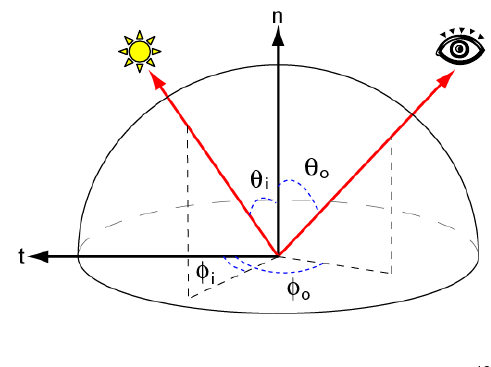
\includegraphics[height=4cm]{slike/brdf.png}
	\end{center}
\end{frame}

\begin{frame}{BRDF}
	\begin{itemize}
		\item Dovodi se veza intenziteta iz svakog smjera s \textsl{odlaznim} svjetlom
		\item \alert{$\mathbf{l}$ smjer dolaznog svjetla, \textsl{incoming}} 
		\item \alert{$\mathbf{v}$ smjer očišta, \textsl{outgoing}} 
	\end{itemize}
	\onslide {
		\begin{align*}
		I_{out}(\mathbf{v}) = I_{in}(\mathbf{l})f_r(\mathbf{v}, \mathbf{l})
		\end{align*}
	}
	\onslide {
		\begin{align*}
		I_{out}\mathbf{v} = I_{svjetlo}\frac{\cos \theta_i}{r^2}f_r(\mathbf{v}, \mathbf{l})
		\end{align*}
	}
	\begin{center}
		\includegraphics[height=3cm]{slike/brdf.png}
	\end{center}
\end{frame}

\begin{frame}{Izotropni vs anizotropni}
	\begin{block}{Izotropni materijal}
		\begin{itemize} %[<+->]
			\item Ako su $\mathbf{l}$ i $\mathbf{v}$ fiksni 
			\item Ako rotacija površine oko normale ne mijenja refleksiju,
		\end{itemize}
	\end{block}	
\end{frame}

\begin{frame}{Parametarski BRDF}
	\begin{itemize} %[<+->]
		\item BRDF se može mjeriti, ali 4D tablice nisu praktične
		\item Parametarski BRDF definiraju vezu između dolaznog i odlaznog svjetla pomoću formule
		\begin{itemize} %[<+->]
			\item Promjena osobina s parametrima, npr. sjajnost
		\end{itemize}
		\item Popularni modeli: Diffuse, Blinn-Phong, Cook-Torrance, Lafortune, Ward, itd.
	\end{itemize}
\end{frame}

\begin{frame}{Now you're just being silly}
	\only<1> {
	\begin{center}
			\includegraphics[height=4.5cm]{slike/slide_043_cropped.jpg}
	\end{center}
	}
\only<2> {
	\begin{center}
		\includegraphics[height=3.5cm]{slike/slide_044_cropped.jpg}
	\end{center}
}
\only<3> {
	\begin{center}
		\includegraphics[height=4.5cm]{slike/slide_045_cropped.jpg}
	\end{center}
}
\only<4> {
	\begin{center}
		\includegraphics[height=3.5cm]{slike/slide_046_cropped.jpg}
	\end{center}
}
\only<5> {
	\begin{center}
		\includegraphics[height=4.5cm]{slike/slide_047_cropped.jpg}
	\end{center}
}\only<6> {
\begin{center}
	\includegraphics[height=2.5cm]{slike/slide_048_cropped.jpg}
\end{center}
}
\only<6> {
	\begin{center}
		\includegraphics[height=3.5cm]{slike/slide_049_cropped.jpg}
	\end{center}
}
\end{frame}

\begin{frame}{Idealna difuzna refleksija}
	\begin{itemize} %[<+->]
		\item Pretpostavlja jednaku refleksiju svjetla u svim smjerovima
		\item Idealna difuzna površina je vrlo hrapava površina na mikroskopskom nivou: kreda, glina
		\item Reflektirano svjetlo ovisi u $\cos$ kuta: Lambertov zakon
	\end{itemize}
\end{frame}

\begin{frame}{Idealna difuzna refleksija}
	\begin{itemize}
		\item Za idealu difuznu refleksiju: BRDF konstanta, $f_r(\mathbf{l}, \mathbf{v}) = const$
		\begin{itemize}
			\item Konstanta: $\rho/\pi$, gdje je $\rho$ \textsl{albedo, albino} ili koeficijent refleksije
			\begin{itemize}
				\item iz lat. \textsl{albus}, bijelo 
				\item $0 \leq \rho \leq 1$, omjer reflektiranog svjetla
			\end{itemize}
			\item Još se naziva difuznom komponentom, $k_d$
		\end{itemize}
	\end{itemize}
	
	\begin{center}
		\begin{tabular}{|c|c|}
			\hline  asfalt& 0.04-0.12 \\ 
			trava &  0.25\\ 
			pijesak, pustinja& 0.4 \\ 
			beton& 0.55 \\ 
			snijeg& 0.8-0.9 \\ 
			\hline 
		\end{tabular} 
		\\
		\includegraphics[height=1.5cm]{slike/albedo.jpg}
	\end{center}
\end{frame}
\begin{frame}{Idealna difuzna refleksija}
	\begin{itemize}
		\item jedan parametar $k_d$ za svaki RGB kanal
	\end{itemize}
	\begin{align*}
	I_d = k_d\max (0, \mathbf{n}\cdot \mathbf{l})\frac{I_i}{r^2}
	\end{align*}
	\begin{columns}[onlytextwidth]
		\begin{column}{0.5\textwidth}
			\begin{itemize}
				\item $k_d$ koeficijent difuzije
				\item $ \mathbf{n}$ normala površine
				\item $  \mathbf{l}$ kut upada svjetla
				\item $I_i$ intenzitet svjetla
				\item $r$ udaljenost površine od izvora svjetla
				\item $I_o$ rezultirajući intenzitet svjetla
				\item \alert{Ne smije se zaboraviti normalizacija vektora $ \mathbf{n}$ i $ \mathbf{l}$ }
			\end{itemize}
		\end{column}
		\begin{column}{0.4\textwidth}
			\begin{center}
				\includegraphics[height=4cm]{slike/diffuse_refl.png}
			\end{center}
		\end{column}
	\end{columns}
	
\end{frame}	

\begin{frame}{Idealna zrcalna\footnote[frame]{specular} refleksija}
	\begin{itemize}
		\item refleksija samo na zrcalnom kutu
		\item Ovisi o položaju očišta	
	\end{itemize}
	\begin{center}
		\includegraphics[height=3cm]{slike/specular_ball.png}
		\includegraphics[height=4cm]{slike/specular_refl.png}
	\end{center}
\end{frame}

\begin{frame}{Zrcalna refleksija}
	\begin{align*}
	\mathbf{R} = -\mathbf{L} + 2 (\mathbf{L}\cdot \mathbf{N})\mathbf{N}
	\end{align*}
	\begin{center}
		\includegraphics[height=3cm]{slike/mirror_refl.png}
	\end{center}
	\begin{itemize} %[<+->]
		\item Svjetlo se reflektira \alert{samo} u zrcalnom smjeru
		\item Dirac delta funkcija pomnožena sa zrcalnim koeficijentom $k_s$ 
		\begin{itemize}
			\item $\delta_a(x) = \frac{1}{a\sqrt{\pi}}e^{-x^2/a^2}$
		\end{itemize}
		\item Nije korisna za točkasti izvor svjelta
		\begin{itemize}
			\item Ne može se vidjeti zrcalna refleksija beskonačno malog svjetla
		\end{itemize}
	\end{itemize}
\end{frame}

\begin{frame}{Realnija refleksija}
	\begin{itemize} %[<+->]
		\item Realni sjajni objekti su značajno drukčiji od idealne zrcalne refleksije
		\item Sjaj je zamućen
		\item Realni objekti nisu idealni difuzni objekti \ldots
	\end{itemize}
	\begin{center}
		\includegraphics[height=3cm]{slike/glossy_material.png}
	\end{center}
\end{frame}

\begin{frame}{Realnija refleksija}
	\begin{itemize} %[<+->]
		\item Jednostavni model za sjajne materijale
		\begin{itemize}
			\item Većina reflektiranog svjetla putuje u smjeru idealne zrcalne zrake
		\end{itemize}
		\item Zbog mikroskopske varijacije površine dio svjetla se reflektira u malo promijenjenom smjeru od idealne zrcalne zrake
		\item Ako se očište kutno pomiče dalje od reflektirane zrake, sve manje se vidi reflektiranog svjetla
	\end{itemize}
	
	\begin{center}
		\includegraphics[height=2cm]{slike/specular_real_refl.png}
	\end{center}
\end{frame}

\begin{frame}{Realnija refleksija, Phong-ov model}
	\begin{itemize} %[<+->]
		\item Koliko svjetla se reflektira?
		\begin{itemize}
			\item Ovisi o kutu $\alpha$ između smjera idealne refleksije $\mathbf{r}$ i smjera gledanja $\mathbf{v}$
			\item $I = k_s\left(\cos \alpha\right)^q\frac{I_i}{r^2} = 
			k_s\left(\mathbf{v}\cdot \mathbf{r}\right)^q\frac{I_i}{r^2}$
		\end{itemize}
	\end{itemize}
	\begin{center}
		\includegraphics[height=3.5cm]{slike/phong_model.png}
	\end{center}
\end{frame}

\begin{frame}{Realnija refleksija, Phong-ov model}
	\begin{itemize}
		\item $q$, utjecaj
	\end{itemize}
	\begin{center}
		\includegraphics[height=3.5cm]{slike/specular_q_coeff.png}
	\end{center}
\end{frame}

\begin{frame}{Phong-ov model}
	\begin{itemize}
		\item Distribucija zrcalne refleksije -> \textsl{lobe}
		\item Phong-ov model ima oblik $ (\mathbf{r}\cdot \mathbf{v})^q$
	\end{itemize}
	\begin{center}
		\includegraphics[height=3.5cm]{slike/phong_model_complete.png}
	\end{center}
\end{frame}

\begin{frame}{Phong-ov model}
	Suma tri komponente:
	\begin{itemize}
		\item idealna difuzna refleksija
		\item zrcalna refleksija
		\item ambijentna komponenta
	\end{itemize}
	\begin{center}
		\includegraphics[height=3.5cm]{slike/phong_model_complete.png}
	\end{center}
\end{frame}
\begin{frame}{Ambijentalna komponenta}
	\begin{block}{}
		$I = k_{a}I_{a}$
		\begin{itemize}
			\item $k_{a}$ - koeficijent reflektirane ambijentne svjetlosti
			\item $I_{a}$ - Intenzitet ambijentne svjetlosti
		\end{itemize}
	\end{block}
	\begin{itemize}
		\item Reflektiranje svih poligona okolnog prostora
		\item Aproksimacija globalnog osvjetljenja
		\item hack
	\end{itemize}
\end{frame}

\begin{frame}{Phong-ov model, sve zajedno}
	\begin{align*}
	I_o = k_aI_i + \left[k_d\left(\mathbf{n}\cdot\mathbf{l}\right)+
	k_s\left(\mathbf{v}\cdot\mathbf{r}\right)^q\right]\frac{I_i}{r^2}
	\end{align*}
	\begin{center}
		\includegraphics[width=11cm]{slike/phong_reflection.png}
		\bigskip
		
		\includegraphics[width=7cm]{slike/phong_constants.png}
	\end{center}
	
\end{frame}

\begin{frame}{Diffuse vs Phong - Call of Duty 4}
	\begin{center}
		\includegraphics[width=5.5cm]{slike/shot0012.jpg}
		\includegraphics[width=5.5cm]{slike/shot0010.jpg}
	\end{center}
\end{frame}

\begin{frame}{Magla}
	\begin{itemize}
		\item Linearna kombinacija izračunatog intenziteta svjetla $I$ i boje magle $c_f$
		\item $d$ je udaljenost objekta (točke na površini objekta) od očišta 
	\end{itemize}
	$$I_f = f(d)I + (1-f(d))c_f$$
	\begin{itemize}
		\item $0 \leq f(d) \leq 1$
		\begin{itemize}
			\item $f(d)=1$ maks vidljivost - boja objekta je originalna
			\item $f(d)=0$ minimalna vidljivost - boja objekta je boja magle
			\item $f(d) = e^{-\rho_{magle}d}$
		\end{itemize}
	\end{itemize}
\end{frame}
\section{Sjenčanje}
\begin{frame}{Sjenčanje vs osvjetljavanje}
	\begin{itemize}%[<+->]
		\item Koliko se sjenčanje razlikuje od osvjetljavanja?
		\item Osvjetljenje se izračunava na svakoj točki na površini objekta
		\item Sjenčanje je \textsl{hack} kojim se računa osvjetljenje samo na verteksima te se interpolira između njih
	\end{itemize}
	\begin{center}
		\includegraphics[width=3cm]{slike/shade_vs_light_01.png}
		\includegraphics[width=3cm]{slike/shade_vs_light_02.png}
	\end{center}
\end{frame}

\begin{frame}{Konstantno sjenčanje}
	\begin{itemize}%[<+->]
		\item Definiramo normalu na svakom poligonu (ne na svakom verteksu)
		\item Osvjetljenje: Izračunava se intenzitet svjetla u centru svakog poligona
		\item Sjenčanje: Svaka uzorkovana točka poligona se je zadana s intepoliranim svjetlom na verteksu (ditto)
	\end{itemize}
	\begin{center}
		\includegraphics[width=3cm]{slike/shade_vs_light_01.png}
	\end{center}
\end{frame}

\begin{frame}{Konstantno sjenčanje}      
	Sve točke unutar jednog poligona imaju isti intenzitet 
	\begin{center}
		\includegraphics[width=7cm]{slike/08_flat_shade.png}
	\end{center}
	\begin{block}{određivanje normala u vrhovima}
		\begin{itemize}
			\item odrediti normale svih poligonalnih površina
			\item izračunati aritmetičku sredinu normala poligona incidentnih s vrhom
		\end{itemize}
	\end{block}
	
	\begin{center}
		\includegraphics[width=7cm]{slike/08_flat_shade2.png}
	\end{center}
\end{frame}

\begin{frame}{Intermezzo - Bilinearna interpolacija}
	Jednostavni oblik bilinearne interpolacije
	\begin{center}
		\includegraphics[height=5cm]{slike/interp_quad.png}
	\end{center}
	\begin{itemize}
		\item Bilinearna interpolacija nije linearna
		\item Produkt linearnih interpolacija
	\end{itemize}
	.
\end{frame}

\begin{frame}{Gouraud sjenčanje}
	\begin{itemize}%[<+->]
		\item Definiramo normalu na svakom verteksu
		\item Osvjetljenje: Evaluirati intenzitet svjetla na svakom verteksu s pridruženom normalom
		\item Sjenčanje: Svaka uzorkovana točka na poligonu se interpolira pomoću vrijednosti verteksa poligona
	\end{itemize}
	\begin{center}
		\includegraphics[width=3cm]{slike/shade_vs_light_01.png}
	\end{center}
\end{frame}
\begin{frame}{Gouraud-ovo sjenčanje}
	\begin{itemize}%[<+->]
		\item U svakom vrhu poligona se računa intenzitet
		\item Dobivene intenzitete linearno interpoliramo
		\item Za sjecišta ispitne linije sa bridovima $Q$ i $R$ interpoliramo duž bridova\\
		$I_{Q}=(1-u)I_{A}+uI_{B}$, za $u=\frac{\overline{AQ}}{\overline{AB}}$\\
		$I_{R}=(1-v)I_{D}+vI_{C}$, za $v=\frac{\overline{DR}}{\overline{DC}}$
		\item Interpoliranje duže poligona \\
		$I_{P}=(1-t)I_{R}+tI_{Q}$, za $t=\frac{\overline{RP}}{\overline{RQ}}$
	\end{itemize}
	\begin{center}
		\includegraphics[width=4cm]{slike/09_gouraud1.png}
		\includegraphics[width=4cm]{slike/09_gouraud2.png}
	\end{center}
\end{frame}
\begin{frame}{Gouraud-ovo sjenčanje}
	\only<1>{Nedostatak: Machov vizualni učinak (svijetle i tamne pruge)
		\begin{center}
			\includegraphics[width=6cm]{slike/09_gouraud3.png}
	\end{center}}
	\only<2>{\begin{center}
			\includegraphics[width=6cm]{slike/09_gouraud4.png}
	\end{center}}
\end{frame}
\begin{frame}{Phong-ovo sjenčanje}
	\begin{itemize} %[<+->]
		\item Svaki verteks ima pridruženu normalu
		\item Osvjetljenje: Evaluirati intenzitet svjetla na svakom verteksu s pridruženom normalom
		\item Sjenčanje: Za svaku točku na poligonu interpoliramo normale pomoću normala verteksa poligona i izračunamo intenzitet osvjetljenja s interpoliranom normalom za svaku uzorkovanu točku poligona
	\end{itemize}
	\begin{center}
		\includegraphics[width=3cm]{slike/shade_vs_light_02.png}
	\end{center}
\end{frame}






\begin{frame}{Phong-ovo sjenčanje}       
	\begin{itemize}%[<+->]
		\item Izračunamo normale u vrhovima
		\item Interpoliramo normale duž bridova
		\item Interpoliramo dobivene normale duž ispitne linije
		\item Izračunamo intenzitet na kraju
	\end{itemize}
\end{frame}


\begin{frame}{Phong-ovo sjenčanje contd. }
	\begin{center}
		\includegraphics[width=5cm]{slike/10_phong1.png}\\
		$\vec{n}_{Q} =(1-u)\vec{n}_{A}+u\vec{n}_{B}$, za $u=\frac{\overline{AQ}}{\overline{AB}}$\\
		$\vec{n}_{R} =(1-v)\vec{n}_{D}+v\vec{n}_{C}$, za $u=\frac{\overline{DR}}{\overline{DC}}$\\
		$\vec{n}_{P} =(1-t)\vec{n}_{R}+t\vec{n}_{Q}$, za $u=\frac{\overline{RP}}{\overline{RQ}}$\\
		$\vec{n}_{P2} =\vec{n}_{P1} + (\vec{n}_{Q}-\vec{n}_{R})(t_{2}-t_{1})$
	\end{center}
\end{frame}

%\begin{frame}{Phong-ovo sjenčanje contd.}
%	\begin{itemize}%[<+->]
%		\item Phong-ovo sjenčanje bolje od Gouraud
%		\item sporije izvršavanje
%		\item umanjuje Machov učinak
%	\end{itemize}
%	Anizotropni učinak
%	\begin{center}
%		\includegraphics[width=4cm]{slike/10_phong2.png}
%	\end{center}
%\end{frame}

%\begin{frame}{Machov učinak}
%	\begin{itemize}
%		\item Machov učinak: iluzija
%		\item Previše se naglašava kontrast između sličnih intenziteta
%		\item Intenzitet unutar svakog kvadrata je isti
%	\end{itemize}
%	
%	\begin{center}
%		\includegraphics[width=5cm]{slike/mach_ucinak.png}
%	\end{center}
%\end{frame}
%
%\begin{frame}
%	\begin{center}
%		\includegraphics[width=8cm]{slike/slide_013_cropped.jpg}
%	\end{center}
%\end{frame}
\plain{Pitanja?}
\end{document}